\section{Sample scatter touched against commit - Repository: 21} 
\begin{figure}
  \centering 
  \begin{subfigure}[b] 
{0.45\textwidth}
    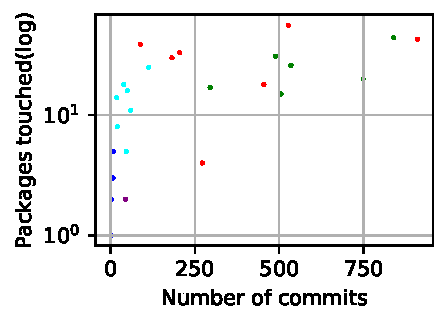
\includegraphics{sections/results/21/packages/sample_scatter_touched_against_commit.packages.sample.first.pdf}
    \caption{packages}
    \label{figure.sections/results/21/packages/sample_scatter_touched_against_commit.packages.sample.first.pdf}
  \end{subfigure}
\vspace{3mm}
  \begin{subfigure}[b] 
{0.45\textwidth}
    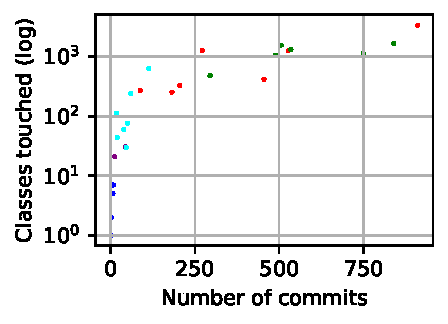
\includegraphics{sections/results/21/classes/sample_scatter_touched_against_commit.classes.sample.first.pdf}
    \caption{classes}
    \label{figure.sections/results/21/classes/sample_scatter_touched_against_commit.classes.sample.first.pdf}
  \end{subfigure}
  \begin{subfigure}[b] 
{0.45\textwidth}
    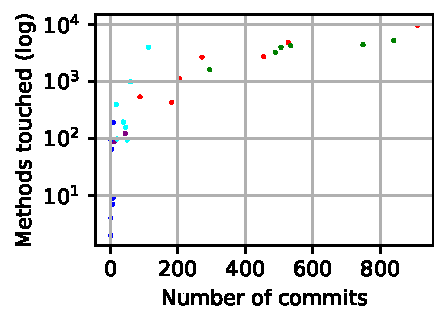
\includegraphics{sections/results/21/methods/sample_scatter_touched_against_commit.methods.sample.first.pdf}
    \caption{methods}
    \label{figure.sections/results/21/methods/sample_scatter_touched_against_commit.methods.sample.first.pdf}
  \end{subfigure}
\caption[Short]{\begin{minipage}[t]{\linewidth}Scatter plots of the log total number of components touched (y-axis) against the number of commits (x-axis) made by samples of developers capped at 84 sustained later joiners from six (6) categories: \color{Blue}Transient Founder (Blue, NUM1), \color{Purple}Moderate Founder (Purple, 3), \color{Green} Sustained Founder (Green, 7), \color{Orange} Transient Later Joiner (Orange, 84), \color{Cyan}Moderate Later Joiner (Cyan, 84), \color{Red} Sustained Later Joiner (Red, 84). \color{Black}\end{minipage}} 
\end{figure}
\clearpage 
\section{Sample scatter touched against commit - Repository: 21} 
\begin{figure}
  \centering 
  \begin{subfigure}[b] 
{0.45\textwidth}
    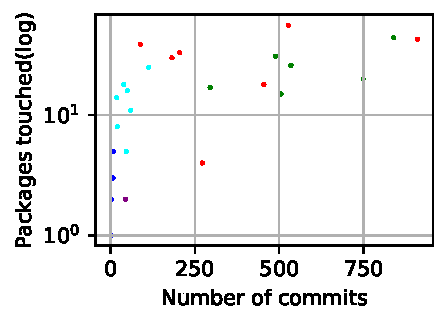
\includegraphics{sections/results/21/packages/sample_scatter_touched_against_commit.packages.sample.first.pdf}
    \caption{packages}
    \label{figure.sections/results/21/packages/sample_scatter_touched_against_commit.packages.sample.first.pdf}
  \end{subfigure}
\vspace{3mm}
  \begin{subfigure}[b] 
{0.45\textwidth}
    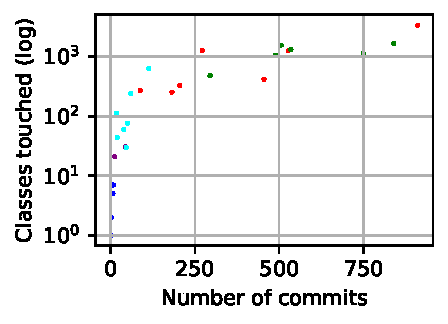
\includegraphics{sections/results/21/classes/sample_scatter_touched_against_commit.classes.sample.first.pdf}
    \caption{classes}
    \label{figure.sections/results/21/classes/sample_scatter_touched_against_commit.classes.sample.first.pdf}
  \end{subfigure}
  \begin{subfigure}[b] 
{0.45\textwidth}
    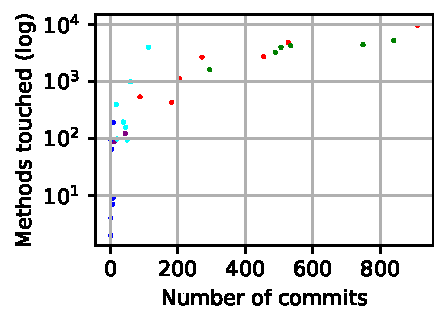
\includegraphics{sections/results/21/methods/sample_scatter_touched_against_commit.methods.sample.first.pdf}
    \caption{methods}
    \label{figure.sections/results/21/methods/sample_scatter_touched_against_commit.methods.sample.first.pdf}
  \end{subfigure}
\caption[Short]{\begin{minipage}[t]{\linewidth}Scatter plots of the log total number of components touched (y-axis) against the number of commits (x-axis) made by samples of developers capped at 84 sustained later joiners from six (6) categories: \color{Blue}Transient Founder (Blue, NUM1), \color{Purple}Moderate Founder (Purple, 3), \color{Green} Sustained Founder (Green, 7), \color{Orange} Transient Later Joiner (Orange, 84), \color{Cyan}Moderate Later Joiner (Cyan, 84), \color{Red} Sustained Later Joiner (Red, 84). \color{Black}\end{minipage}} 
\end{figure}
\clearpage 
\section{Sample scatter touched against commit - Repository: 21} 
\begin{figure}
  \centering 
  \begin{subfigure}[b] 
{0.45\textwidth}
    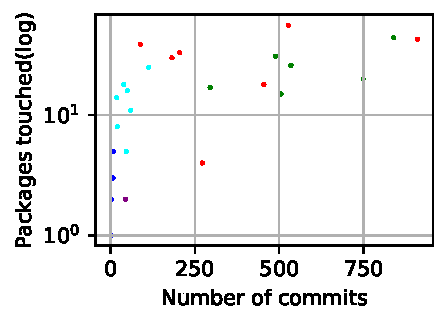
\includegraphics{sections/results/21/packages/sample_scatter_touched_against_commit.packages.sample.first.pdf}
    \caption{packages}
    \label{figure.sections/results/21/packages/sample_scatter_touched_against_commit.packages.sample.first.pdf}
  \end{subfigure}
\vspace{3mm}
  \begin{subfigure}[b] 
{0.45\textwidth}
    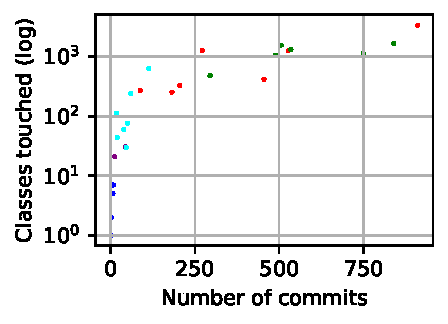
\includegraphics{sections/results/21/classes/sample_scatter_touched_against_commit.classes.sample.first.pdf}
    \caption{classes}
    \label{figure.sections/results/21/classes/sample_scatter_touched_against_commit.classes.sample.first.pdf}
  \end{subfigure}
  \begin{subfigure}[b] 
{0.45\textwidth}
    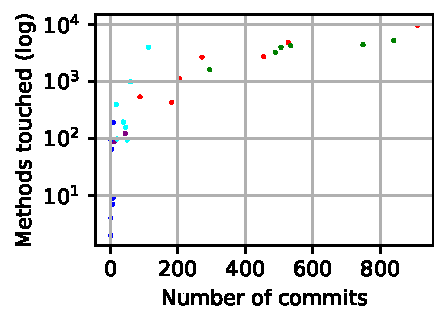
\includegraphics{sections/results/21/methods/sample_scatter_touched_against_commit.methods.sample.first.pdf}
    \caption{methods}
    \label{figure.sections/results/21/methods/sample_scatter_touched_against_commit.methods.sample.first.pdf}
  \end{subfigure}
\caption[Short]{\begin{minipage}[t]{\linewidth}Scatter plots of the log total number of components touched (y-axis) against the number of commits (x-axis) made by samples of developers capped at 84 sustained later joiners from six (6) categories: \color{Blue}Transient Founder (Blue, NUM1), \color{Purple}Moderate Founder (Purple, 3), \color{Green} Sustained Founder (Green, 7), \color{Orange} Transient Later Joiner (Orange, 84), \color{Cyan}Moderate Later Joiner (Cyan, 84), \color{Red} Sustained Later Joiner (Red, 84). \color{Black}\end{minipage}} 
\end{figure}
\clearpage 
\section{Sample scatter touched against commit - Repository: 21} 
\begin{figure}
  \centering 
  \begin{subfigure}[b] 
{0.45\textwidth}
    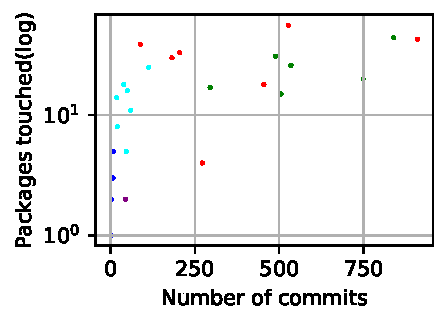
\includegraphics{sections/results/21/packages/sample_scatter_touched_against_commit.packages.sample.first.pdf}
    \caption{packages}
    \label{figure.sections/results/21/packages/sample_scatter_touched_against_commit.packages.sample.first.pdf}
  \end{subfigure}
\vspace{3mm}
  \begin{subfigure}[b] 
{0.45\textwidth}
    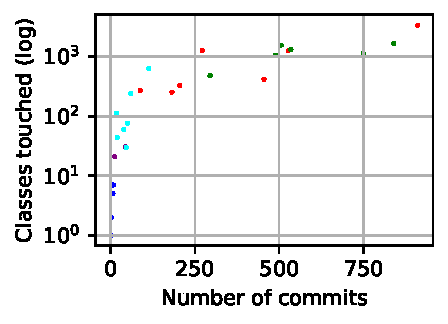
\includegraphics{sections/results/21/classes/sample_scatter_touched_against_commit.classes.sample.first.pdf}
    \caption{classes}
    \label{figure.sections/results/21/classes/sample_scatter_touched_against_commit.classes.sample.first.pdf}
  \end{subfigure}
  \begin{subfigure}[b] 
{0.45\textwidth}
    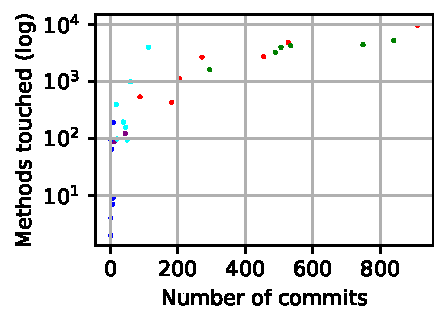
\includegraphics{sections/results/21/methods/sample_scatter_touched_against_commit.methods.sample.first.pdf}
    \caption{methods}
    \label{figure.sections/results/21/methods/sample_scatter_touched_against_commit.methods.sample.first.pdf}
  \end{subfigure}
\caption[Short]{\begin{minipage}[t]{\linewidth}Scatter plots of the log total number of components touched (y-axis) against the number of commits (x-axis) made by samples of developers capped at 84 sustained later joiners from six (6) categories: \color{Blue}Transient Founder (Blue, NUM1), \color{Purple}Moderate Founder (Purple, 3), \color{Green} Sustained Founder (Green, 7), \color{Orange} Transient Later Joiner (Orange, 84), \color{Cyan}Moderate Later Joiner (Cyan, 84), \color{Red} Sustained Later Joiner (Red, 84). \color{Black}\end{minipage}} 
\end{figure}
\clearpage 
\section{Sample scatter touched against commit - Repository: 21} 
\begin{figure}
  \centering 
  \begin{subfigure}[b] 
{0.45\textwidth}
    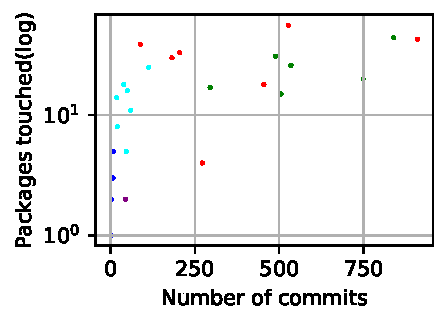
\includegraphics{sections/results/21/packages/sample_scatter_touched_against_commit.packages.sample.first.pdf}
    \caption{packages}
    \label{figure.sections/results/21/packages/sample_scatter_touched_against_commit.packages.sample.first.pdf}
  \end{subfigure}
\vspace{3mm}
  \begin{subfigure}[b] 
{0.45\textwidth}
    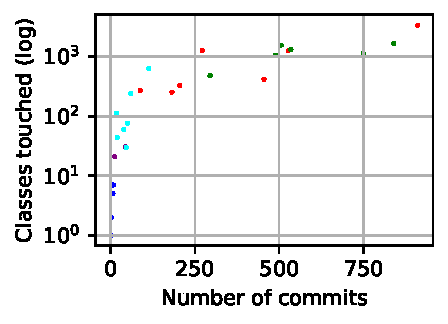
\includegraphics{sections/results/21/classes/sample_scatter_touched_against_commit.classes.sample.first.pdf}
    \caption{classes}
    \label{figure.sections/results/21/classes/sample_scatter_touched_against_commit.classes.sample.first.pdf}
  \end{subfigure}
  \begin{subfigure}[b] 
{0.45\textwidth}
    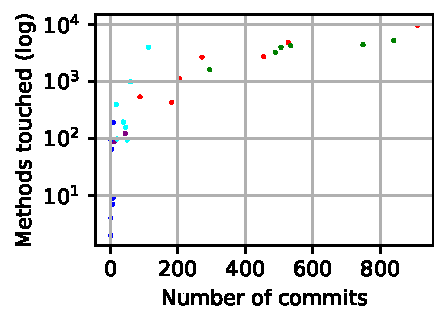
\includegraphics{sections/results/21/methods/sample_scatter_touched_against_commit.methods.sample.first.pdf}
    \caption{methods}
    \label{figure.sections/results/21/methods/sample_scatter_touched_against_commit.methods.sample.first.pdf}
  \end{subfigure}
\caption[Short]{\begin{minipage}[t]{\linewidth}Scatter plots of the log total number of components touched (y-axis) against the number of commits (x-axis) made by samples of developers capped at 84 sustained later joiners from six (6) categories: \color{Blue}Transient Founder (Blue, NUM1), \color{Purple}Moderate Founder (Purple, 3), \color{Green} Sustained Founder (Green, 7), \color{Orange} Transient Later Joiner (Orange, 84), \color{Cyan}Moderate Later Joiner (Cyan, 84), \color{Red} Sustained Later Joiner (Red, 84). \color{Black}\end{minipage}} 
\end{figure}
\clearpage 
\section{Sample scatter touched against commit - Repository: 21} 
\begin{figure}
  \centering 
  \begin{subfigure}[b] 
{0.45\textwidth}
    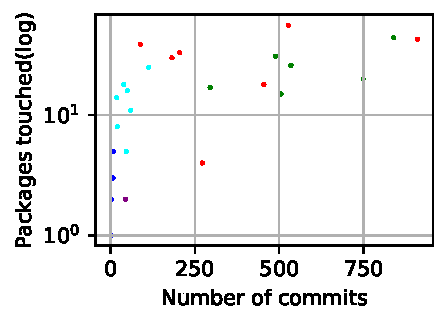
\includegraphics{sections/results/21/packages/sample_scatter_touched_against_commit.packages.sample.first.pdf}
    \caption{packages}
    \label{figure.sections/results/21/packages/sample_scatter_touched_against_commit.packages.sample.first.pdf}
  \end{subfigure}
\vspace{3mm}
  \begin{subfigure}[b] 
{0.45\textwidth}
    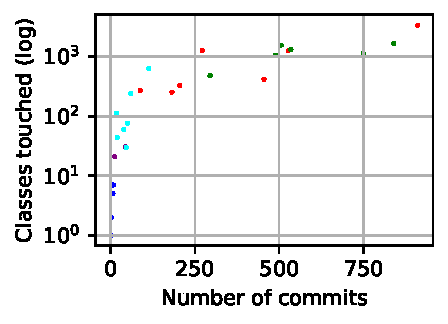
\includegraphics{sections/results/21/classes/sample_scatter_touched_against_commit.classes.sample.first.pdf}
    \caption{classes}
    \label{figure.sections/results/21/classes/sample_scatter_touched_against_commit.classes.sample.first.pdf}
  \end{subfigure}
  \begin{subfigure}[b] 
{0.45\textwidth}
    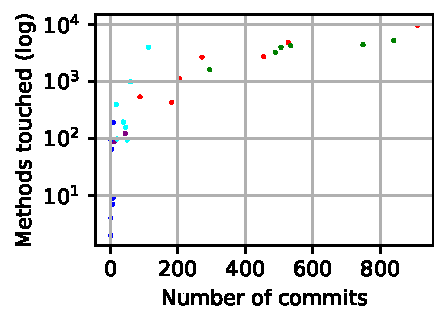
\includegraphics{sections/results/21/methods/sample_scatter_touched_against_commit.methods.sample.first.pdf}
    \caption{methods}
    \label{figure.sections/results/21/methods/sample_scatter_touched_against_commit.methods.sample.first.pdf}
  \end{subfigure}
\caption[Short]{\begin{minipage}[t]{\linewidth}Scatter plots of the log total number of components touched (y-axis) against the number of commits (x-axis) made by samples of developers capped at 84 sustained later joiners from six (6) categories: \color{Blue}Transient Founder (Blue, NUM1), \color{Purple}Moderate Founder (Purple, 3), \color{Green} Sustained Founder (Green, 7), \color{Orange} Transient Later Joiner (Orange, 84), \color{Cyan}Moderate Later Joiner (Cyan, 84), \color{Red} Sustained Later Joiner (Red, 84). \color{Black}\end{minipage}} 
\end{figure}
\clearpage 
\section{Sample scatter touched against commit - Repository: 21} 
\begin{figure}
  \centering 
  \begin{subfigure}[b] 
{0.45\textwidth}
    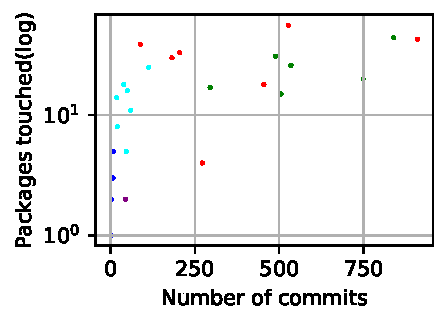
\includegraphics{sections/results/21/packages/sample_scatter_touched_against_commit.packages.sample.first.pdf}
    \caption{packages}
    \label{figure.sections/results/21/packages/sample_scatter_touched_against_commit.packages.sample.first.pdf}
  \end{subfigure}
\vspace{3mm}
  \begin{subfigure}[b] 
{0.45\textwidth}
    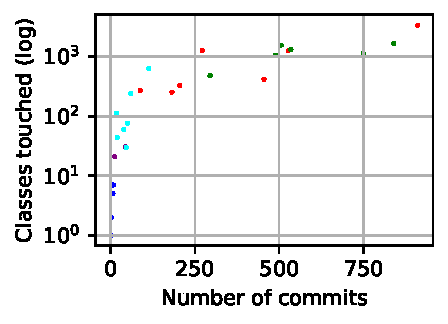
\includegraphics{sections/results/21/classes/sample_scatter_touched_against_commit.classes.sample.first.pdf}
    \caption{classes}
    \label{figure.sections/results/21/classes/sample_scatter_touched_against_commit.classes.sample.first.pdf}
  \end{subfigure}
  \begin{subfigure}[b] 
{0.45\textwidth}
    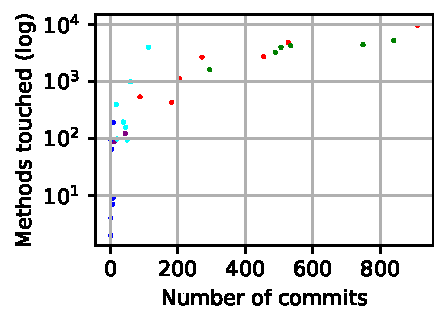
\includegraphics{sections/results/21/methods/sample_scatter_touched_against_commit.methods.sample.first.pdf}
    \caption{methods}
    \label{figure.sections/results/21/methods/sample_scatter_touched_against_commit.methods.sample.first.pdf}
  \end{subfigure}
\caption[Short]{\begin{minipage}[t]{\linewidth}Scatter plots of the log total number of components touched (y-axis) against the number of commits (x-axis) made by samples of developers capped at 84 sustained later joiners from six (6) categories: \color{Blue}Transient Founder (Blue, NUM1), \color{Purple}Moderate Founder (Purple, 3), \color{Green} Sustained Founder (Green, 7), \color{Orange} Transient Later Joiner (Orange, 84), \color{Cyan}Moderate Later Joiner (Cyan, 84), \color{Red} Sustained Later Joiner (Red, 84). \color{Black}\end{minipage}} 
\end{figure}
\clearpage 
\section{Sample scatter touched against commit - Repository: 21} 
\begin{figure}
  \centering 
  \begin{subfigure}[b] 
{0.45\textwidth}
    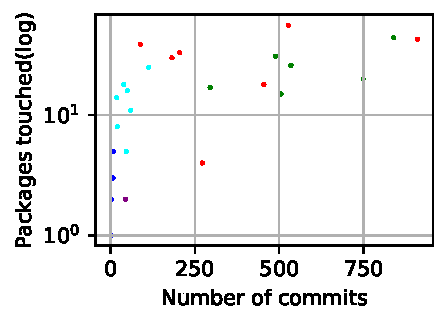
\includegraphics{sections/results/21/packages/sample_scatter_touched_against_commit.packages.sample.first.pdf}
    \caption{packages}
    \label{figure.sections/results/21/packages/sample_scatter_touched_against_commit.packages.sample.first.pdf}
  \end{subfigure}
\vspace{3mm}
  \begin{subfigure}[b] 
{0.45\textwidth}
    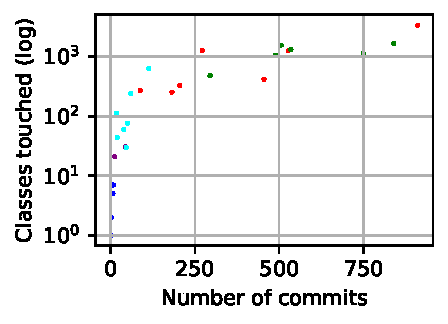
\includegraphics{sections/results/21/classes/sample_scatter_touched_against_commit.classes.sample.first.pdf}
    \caption{classes}
    \label{figure.sections/results/21/classes/sample_scatter_touched_against_commit.classes.sample.first.pdf}
  \end{subfigure}
  \begin{subfigure}[b] 
{0.45\textwidth}
    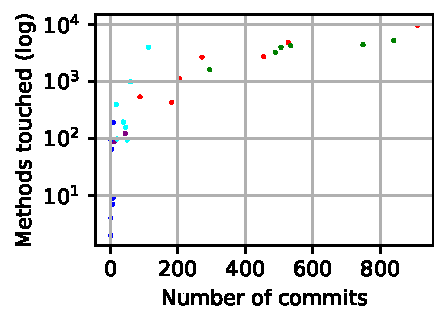
\includegraphics{sections/results/21/methods/sample_scatter_touched_against_commit.methods.sample.first.pdf}
    \caption{methods}
    \label{figure.sections/results/21/methods/sample_scatter_touched_against_commit.methods.sample.first.pdf}
  \end{subfigure}
\caption[Short]{\begin{minipage}[t]{\linewidth}Scatter plots of the log total number of components touched (y-axis) against the number of commits (x-axis) made by samples of developers capped at 84 sustained later joiners from six (6) categories: \color{Blue}Transient Founder (Blue, NUM1), \color{Purple}Moderate Founder (Purple, 3), \color{Green} Sustained Founder (Green, 7), \color{Orange} Transient Later Joiner (Orange, 84), \color{Cyan}Moderate Later Joiner (Cyan, 84), \color{Red} Sustained Later Joiner (Red, 84). \color{Black}\end{minipage}} 
\end{figure}
\clearpage 
\section{Sample scatter touched against commit - Repository: 21} 
\begin{figure}
  \centering 
  \begin{subfigure}[b] 
{0.45\textwidth}
    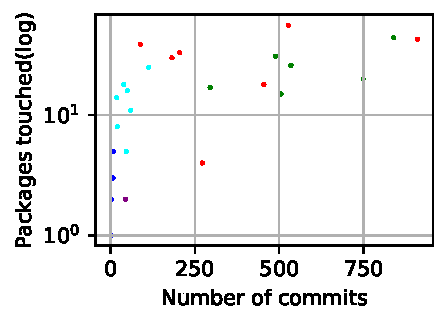
\includegraphics{sections/results/21/packages/sample_scatter_touched_against_commit.packages.sample.first.pdf}
    \caption{packages}
    \label{figure.sections/results/21/packages/sample_scatter_touched_against_commit.packages.sample.first.pdf}
  \end{subfigure}
\vspace{3mm}
  \begin{subfigure}[b] 
{0.45\textwidth}
    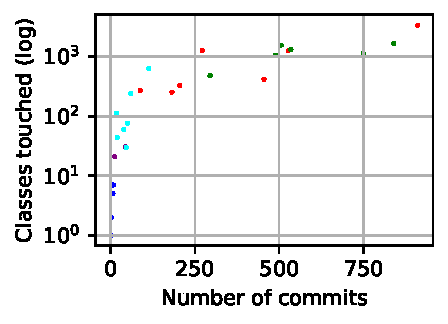
\includegraphics{sections/results/21/classes/sample_scatter_touched_against_commit.classes.sample.first.pdf}
    \caption{classes}
    \label{figure.sections/results/21/classes/sample_scatter_touched_against_commit.classes.sample.first.pdf}
  \end{subfigure}
  \begin{subfigure}[b] 
{0.45\textwidth}
    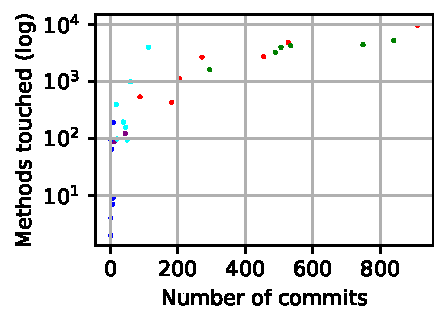
\includegraphics{sections/results/21/methods/sample_scatter_touched_against_commit.methods.sample.first.pdf}
    \caption{methods}
    \label{figure.sections/results/21/methods/sample_scatter_touched_against_commit.methods.sample.first.pdf}
  \end{subfigure}
\caption[Short]{\begin{minipage}[t]{\linewidth}Scatter plots of the log total number of components touched (y-axis) against the number of commits (x-axis) made by samples of developers capped at 84 sustained later joiners from six (6) categories: \color{Blue}Transient Founder (Blue, NUM1), \color{Purple}Moderate Founder (Purple, 3), \color{Green} Sustained Founder (Green, 7), \color{Orange} Transient Later Joiner (Orange, 84), \color{Cyan}Moderate Later Joiner (Cyan, 84), \color{Red} Sustained Later Joiner (Red, 84). \color{Black}\end{minipage}} 
\end{figure}
\clearpage 
\section{Sample scatter touched against commit - Repository: 21} 
\begin{figure}
  \centering 
  \begin{subfigure}[b] 
{0.45\textwidth}
    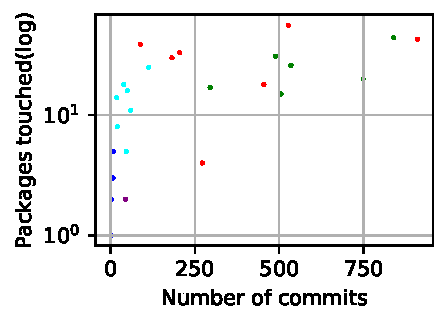
\includegraphics{sections/results/21/packages/sample_scatter_touched_against_commit.packages.sample.first.pdf}
    \caption{packages}
    \label{figure.sections/results/21/packages/sample_scatter_touched_against_commit.packages.sample.first.pdf}
  \end{subfigure}
\vspace{3mm}
  \begin{subfigure}[b] 
{0.45\textwidth}
    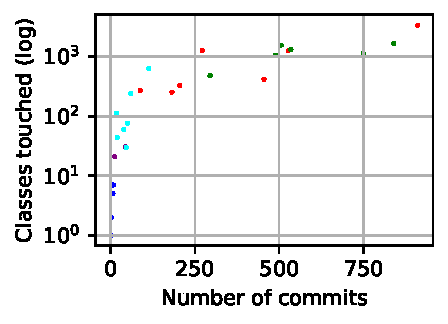
\includegraphics{sections/results/21/classes/sample_scatter_touched_against_commit.classes.sample.first.pdf}
    \caption{classes}
    \label{figure.sections/results/21/classes/sample_scatter_touched_against_commit.classes.sample.first.pdf}
  \end{subfigure}
  \begin{subfigure}[b] 
{0.45\textwidth}
    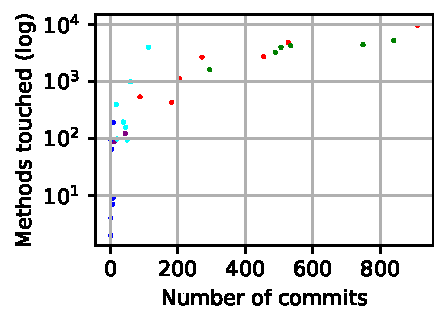
\includegraphics{sections/results/21/methods/sample_scatter_touched_against_commit.methods.sample.first.pdf}
    \caption{methods}
    \label{figure.sections/results/21/methods/sample_scatter_touched_against_commit.methods.sample.first.pdf}
  \end{subfigure}
\caption[Short]{\begin{minipage}[t]{\linewidth}Scatter plots of the log total number of components touched (y-axis) against the number of commits (x-axis) made by samples of developers capped at 84 sustained later joiners from six (6) categories: \color{Blue}Transient Founder (Blue, NUM1), \color{Purple}Moderate Founder (Purple, 3), \color{Green} Sustained Founder (Green, 7), \color{Orange} Transient Later Joiner (Orange, 84), \color{Cyan}Moderate Later Joiner (Cyan, 84), \color{Red} Sustained Later Joiner (Red, 84). \color{Black}\end{minipage}} 
\end{figure}
\clearpage 
\section{Sample scatter touched against commit - Repository: 21} 
\begin{figure}
  \centering 
  \begin{subfigure}[b] 
{0.45\textwidth}
    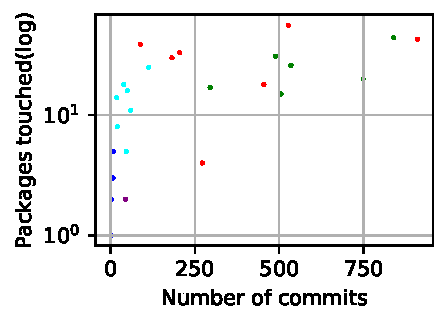
\includegraphics{sections/results/21/packages/sample_scatter_touched_against_commit.packages.sample.first.pdf}
    \caption{packages}
    \label{figure.sections/results/21/packages/sample_scatter_touched_against_commit.packages.sample.first.pdf}
  \end{subfigure}
\vspace{3mm}
  \begin{subfigure}[b] 
{0.45\textwidth}
    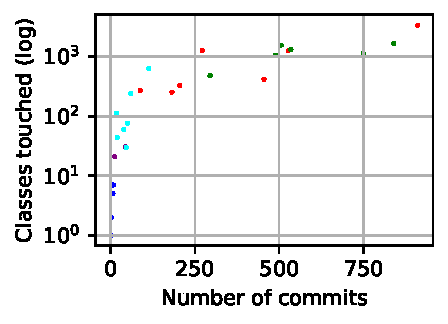
\includegraphics{sections/results/21/classes/sample_scatter_touched_against_commit.classes.sample.first.pdf}
    \caption{classes}
    \label{figure.sections/results/21/classes/sample_scatter_touched_against_commit.classes.sample.first.pdf}
  \end{subfigure}
  \begin{subfigure}[b] 
{0.45\textwidth}
    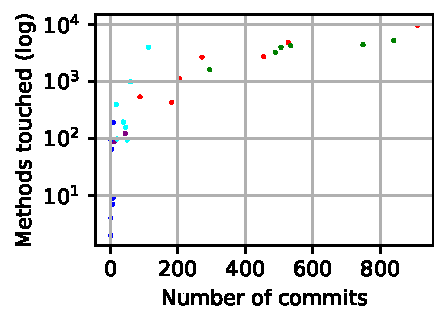
\includegraphics{sections/results/21/methods/sample_scatter_touched_against_commit.methods.sample.first.pdf}
    \caption{methods}
    \label{figure.sections/results/21/methods/sample_scatter_touched_against_commit.methods.sample.first.pdf}
  \end{subfigure}
\caption[Short]{\begin{minipage}[t]{\linewidth}Scatter plots of the log total number of components touched (y-axis) against the number of commits (x-axis) made by samples of developers capped at 84 sustained later joiners from six (6) categories: \color{Blue}Transient Founder (Blue, NUM1), \color{Purple}Moderate Founder (Purple, 3), \color{Green} Sustained Founder (Green, 7), \color{Orange} Transient Later Joiner (Orange, 84), \color{Cyan}Moderate Later Joiner (Cyan, 84), \color{Red} Sustained Later Joiner (Red, 84). \color{Black}\end{minipage}} 
\end{figure}
\clearpage 
\section{Sample scatter touched against commit - Repository: 21} 
\begin{figure}
  \centering 
  \begin{subfigure}[b] 
{0.45\textwidth}
    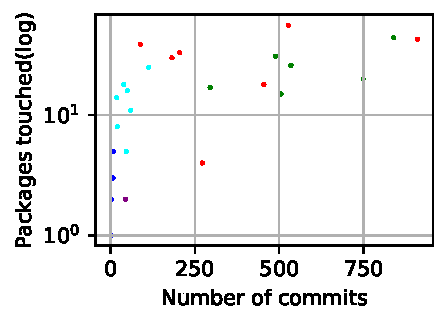
\includegraphics{sections/results/21/packages/sample_scatter_touched_against_commit.packages.sample.first.pdf}
    \caption{packages}
    \label{figure.sections/results/21/packages/sample_scatter_touched_against_commit.packages.sample.first.pdf}
  \end{subfigure}
\vspace{3mm}
  \begin{subfigure}[b] 
{0.45\textwidth}
    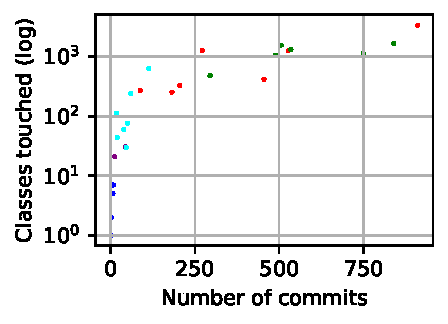
\includegraphics{sections/results/21/classes/sample_scatter_touched_against_commit.classes.sample.first.pdf}
    \caption{classes}
    \label{figure.sections/results/21/classes/sample_scatter_touched_against_commit.classes.sample.first.pdf}
  \end{subfigure}
  \begin{subfigure}[b] 
{0.45\textwidth}
    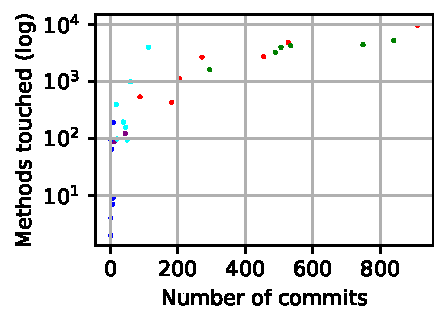
\includegraphics{sections/results/21/methods/sample_scatter_touched_against_commit.methods.sample.first.pdf}
    \caption{methods}
    \label{figure.sections/results/21/methods/sample_scatter_touched_against_commit.methods.sample.first.pdf}
  \end{subfigure}
\caption[Short]{\begin{minipage}[t]{\linewidth}Scatter plots of the log total number of components touched (y-axis) against the number of commits (x-axis) made by samples of developers capped at 84 sustained later joiners from six (6) categories: \color{Blue}Transient Founder (Blue, NUM1), \color{Purple}Moderate Founder (Purple, 3), \color{Green} Sustained Founder (Green, 7), \color{Orange} Transient Later Joiner (Orange, 84), \color{Cyan}Moderate Later Joiner (Cyan, 84), \color{Red} Sustained Later Joiner (Red, 84). \color{Black}\end{minipage}} 
\end{figure}
\clearpage 
\section{Sample scatter touched against commit - Repository: 21} 
\begin{figure}
  \centering 
  \begin{subfigure}[b] 
{0.45\textwidth}
    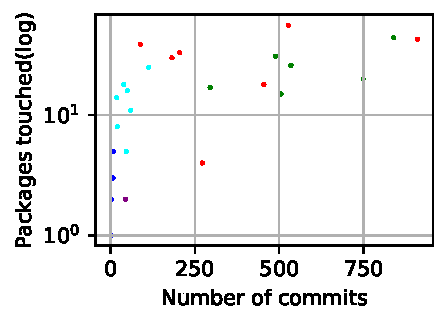
\includegraphics{sections/results/21/packages/sample_scatter_touched_against_commit.packages.sample.first.pdf}
    \caption{packages}
    \label{figure.sections/results/21/packages/sample_scatter_touched_against_commit.packages.sample.first.pdf}
  \end{subfigure}
\vspace{3mm}
  \begin{subfigure}[b] 
{0.45\textwidth}
    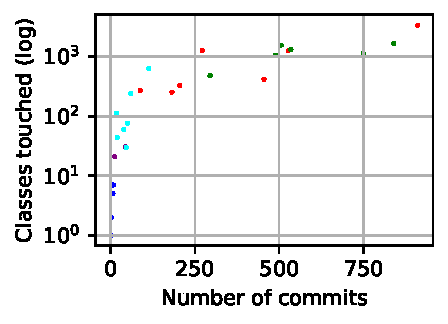
\includegraphics{sections/results/21/classes/sample_scatter_touched_against_commit.classes.sample.first.pdf}
    \caption{classes}
    \label{figure.sections/results/21/classes/sample_scatter_touched_against_commit.classes.sample.first.pdf}
  \end{subfigure}
  \begin{subfigure}[b] 
{0.45\textwidth}
    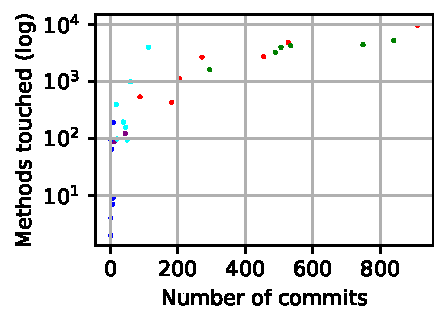
\includegraphics{sections/results/21/methods/sample_scatter_touched_against_commit.methods.sample.first.pdf}
    \caption{methods}
    \label{figure.sections/results/21/methods/sample_scatter_touched_against_commit.methods.sample.first.pdf}
  \end{subfigure}
\caption[Short]{\begin{minipage}[t]{\linewidth}Scatter plots of the log total number of components touched (y-axis) against the number of commits (x-axis) made by samples of developers capped at 84 sustained later joiners from six (6) categories: \color{Blue}Transient Founder (Blue, NUM1), \color{Purple}Moderate Founder (Purple, 3), \color{Green} Sustained Founder (Green, 7), \color{Orange} Transient Later Joiner (Orange, 84), \color{Cyan}Moderate Later Joiner (Cyan, 84), \color{Red} Sustained Later Joiner (Red, 84). \color{Black}\end{minipage}} 
\end{figure}
\clearpage 
\section{Sample scatter touched against commit - Repository: 21} 
\begin{figure}
  \centering 
  \begin{subfigure}[b] 
{0.45\textwidth}
    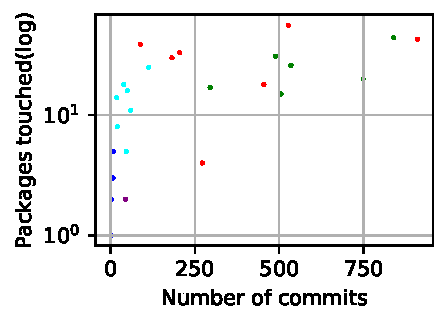
\includegraphics{sections/results/21/packages/sample_scatter_touched_against_commit.packages.sample.first.pdf}
    \caption{packages}
    \label{figure.sections/results/21/packages/sample_scatter_touched_against_commit.packages.sample.first.pdf}
  \end{subfigure}
\vspace{3mm}
  \begin{subfigure}[b] 
{0.45\textwidth}
    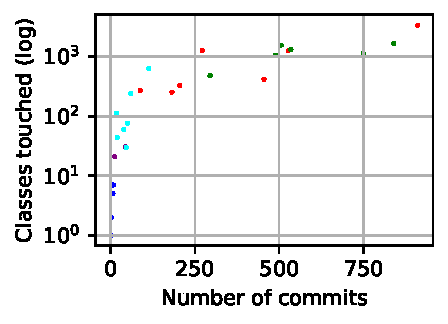
\includegraphics{sections/results/21/classes/sample_scatter_touched_against_commit.classes.sample.first.pdf}
    \caption{classes}
    \label{figure.sections/results/21/classes/sample_scatter_touched_against_commit.classes.sample.first.pdf}
  \end{subfigure}
  \begin{subfigure}[b] 
{0.45\textwidth}
    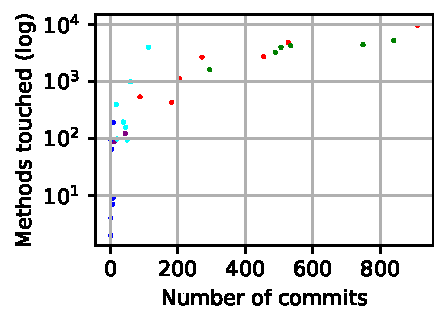
\includegraphics{sections/results/21/methods/sample_scatter_touched_against_commit.methods.sample.first.pdf}
    \caption{methods}
    \label{figure.sections/results/21/methods/sample_scatter_touched_against_commit.methods.sample.first.pdf}
  \end{subfigure}
\caption[Short]{\begin{minipage}[t]{\linewidth}Scatter plots of the log total number of components touched (y-axis) against the number of commits (x-axis) made by samples of developers capped at 84 sustained later joiners from six (6) categories: \color{Blue}Transient Founder (Blue, NUM1), \color{Purple}Moderate Founder (Purple, 3), \color{Green} Sustained Founder (Green, 7), \color{Orange} Transient Later Joiner (Orange, 84), \color{Cyan}Moderate Later Joiner (Cyan, 84), \color{Red} Sustained Later Joiner (Red, 84). \color{Black}\end{minipage}} 
\end{figure}
\clearpage 
\section{Sample scatter touched against commit - Repository: 21} 
\begin{figure}
  \centering 
  \begin{subfigure}[b] 
{0.45\textwidth}
    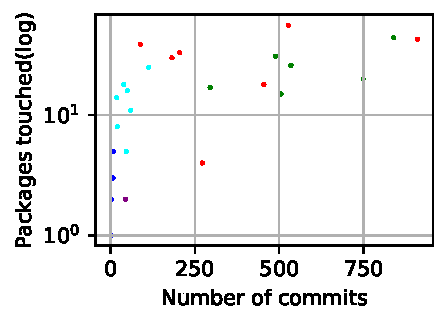
\includegraphics{sections/results/21/packages/sample_scatter_touched_against_commit.packages.sample.first.pdf}
    \caption{packages}
    \label{figure.sections/results/21/packages/sample_scatter_touched_against_commit.packages.sample.first.pdf}
  \end{subfigure}
\vspace{3mm}
  \begin{subfigure}[b] 
{0.45\textwidth}
    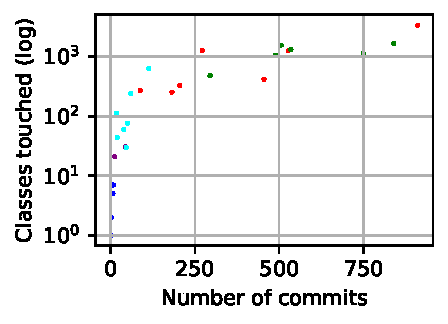
\includegraphics{sections/results/21/classes/sample_scatter_touched_against_commit.classes.sample.first.pdf}
    \caption{classes}
    \label{figure.sections/results/21/classes/sample_scatter_touched_against_commit.classes.sample.first.pdf}
  \end{subfigure}
  \begin{subfigure}[b] 
{0.45\textwidth}
    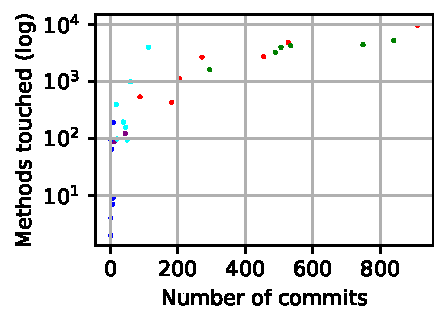
\includegraphics{sections/results/21/methods/sample_scatter_touched_against_commit.methods.sample.first.pdf}
    \caption{methods}
    \label{figure.sections/results/21/methods/sample_scatter_touched_against_commit.methods.sample.first.pdf}
  \end{subfigure}
\caption[Short]{\begin{minipage}[t]{\linewidth}Scatter plots of the log total number of components touched (y-axis) against the number of commits (x-axis) made by samples of developers capped at 84 sustained later joiners from six (6) categories: \color{Blue}Transient Founder (Blue, NUM1), \color{Purple}Moderate Founder (Purple, 3), \color{Green} Sustained Founder (Green, 7), \color{Orange} Transient Later Joiner (Orange, 84), \color{Cyan}Moderate Later Joiner (Cyan, 84), \color{Red} Sustained Later Joiner (Red, 84). \color{Black}\end{minipage}} 
\end{figure}
\clearpage 
\section{Sample scatter touched against commit - Repository: 21} 
\begin{figure}
  \centering 
  \begin{subfigure}[b] 
{0.45\textwidth}
    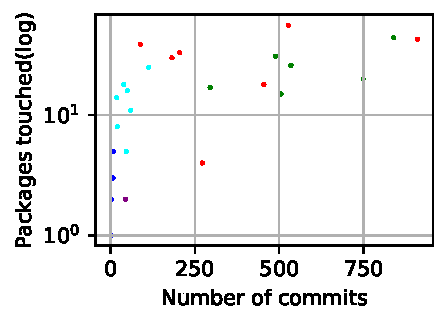
\includegraphics{sections/results/21/packages/sample_scatter_touched_against_commit.packages.sample.first.pdf}
    \caption{packages}
    \label{figure.sections/results/21/packages/sample_scatter_touched_against_commit.packages.sample.first.pdf}
  \end{subfigure}
\vspace{3mm}
  \begin{subfigure}[b] 
{0.45\textwidth}
    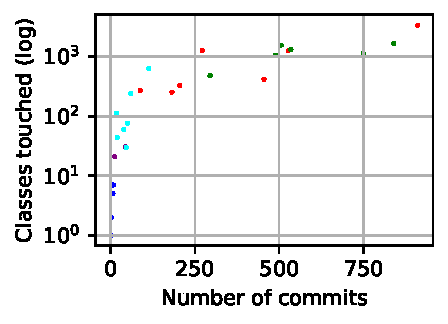
\includegraphics{sections/results/21/classes/sample_scatter_touched_against_commit.classes.sample.first.pdf}
    \caption{classes}
    \label{figure.sections/results/21/classes/sample_scatter_touched_against_commit.classes.sample.first.pdf}
  \end{subfigure}
  \begin{subfigure}[b] 
{0.45\textwidth}
    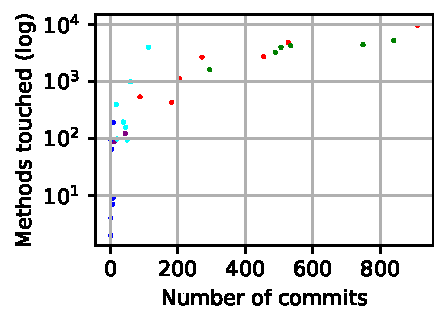
\includegraphics{sections/results/21/methods/sample_scatter_touched_against_commit.methods.sample.first.pdf}
    \caption{methods}
    \label{figure.sections/results/21/methods/sample_scatter_touched_against_commit.methods.sample.first.pdf}
  \end{subfigure}
\caption[Short]{\begin{minipage}[t]{\linewidth}Scatter plots of the log total number of components touched (y-axis) against the number of commits (x-axis) made by samples of developers capped at 84 sustained later joiners from six (6) categories: \color{Blue}Transient Founder (Blue, NUM1), \color{Purple}Moderate Founder (Purple, 3), \color{Green} Sustained Founder (Green, 7), \color{Orange} Transient Later Joiner (Orange, 84), \color{Cyan}Moderate Later Joiner (Cyan, 84), \color{Red} Sustained Later Joiner (Red, 84). \color{Black}\end{minipage}} 
\end{figure}
\clearpage 
\section{Sample scatter touched against commit - Repository: 21} 
\begin{figure}
  \centering 
  \begin{subfigure}[b] 
{0.45\textwidth}
    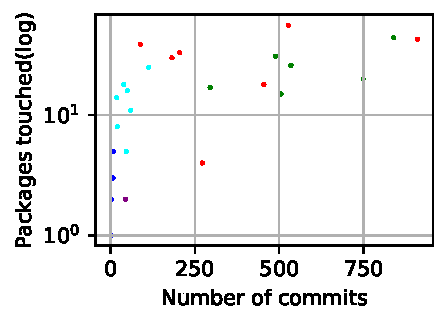
\includegraphics{sections/results/21/packages/sample_scatter_touched_against_commit.packages.sample.first.pdf}
    \caption{packages}
    \label{figure.sections/results/21/packages/sample_scatter_touched_against_commit.packages.sample.first.pdf}
  \end{subfigure}
\vspace{3mm}
  \begin{subfigure}[b] 
{0.45\textwidth}
    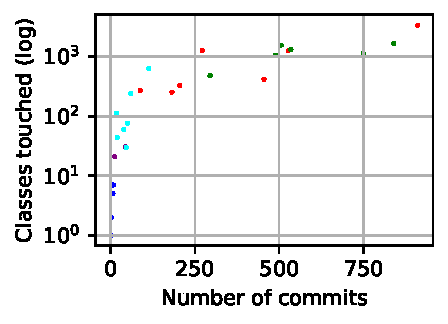
\includegraphics{sections/results/21/classes/sample_scatter_touched_against_commit.classes.sample.first.pdf}
    \caption{classes}
    \label{figure.sections/results/21/classes/sample_scatter_touched_against_commit.classes.sample.first.pdf}
  \end{subfigure}
  \begin{subfigure}[b] 
{0.45\textwidth}
    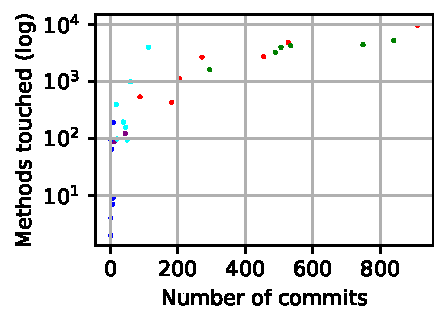
\includegraphics{sections/results/21/methods/sample_scatter_touched_against_commit.methods.sample.first.pdf}
    \caption{methods}
    \label{figure.sections/results/21/methods/sample_scatter_touched_against_commit.methods.sample.first.pdf}
  \end{subfigure}
\caption[Short]{\begin{minipage}[t]{\linewidth}Scatter plots of the log total number of components touched (y-axis) against the number of commits (x-axis) made by samples of developers capped at 84 sustained later joiners from six (6) categories: \color{Blue}Transient Founder (Blue, NUM1), \color{Purple}Moderate Founder (Purple, 3), \color{Green} Sustained Founder (Green, 7), \color{Orange} Transient Later Joiner (Orange, 84), \color{Cyan}Moderate Later Joiner (Cyan, 84), \color{Red} Sustained Later Joiner (Red, 84). \color{Black}\end{minipage}} 
\end{figure}
\clearpage 
\section{Sample scatter touched against commit - Repository: 21} 
\begin{figure}
  \centering 
  \begin{subfigure}[b] 
{0.45\textwidth}
    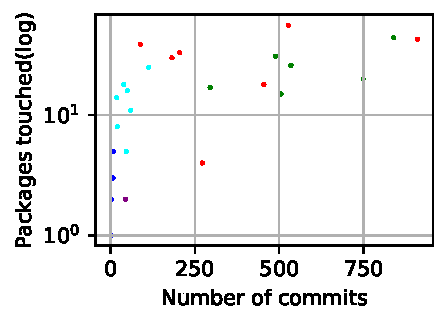
\includegraphics{sections/results/21/packages/sample_scatter_touched_against_commit.packages.sample.first.pdf}
    \caption{packages}
    \label{figure.sections/results/21/packages/sample_scatter_touched_against_commit.packages.sample.first.pdf}
  \end{subfigure}
\vspace{3mm}
  \begin{subfigure}[b] 
{0.45\textwidth}
    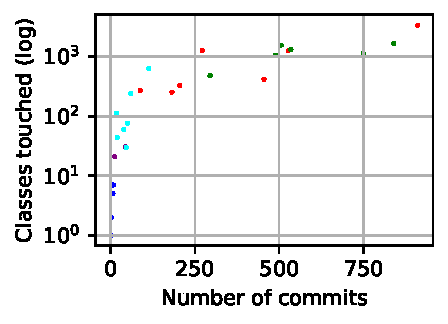
\includegraphics{sections/results/21/classes/sample_scatter_touched_against_commit.classes.sample.first.pdf}
    \caption{classes}
    \label{figure.sections/results/21/classes/sample_scatter_touched_against_commit.classes.sample.first.pdf}
  \end{subfigure}
  \begin{subfigure}[b] 
{0.45\textwidth}
    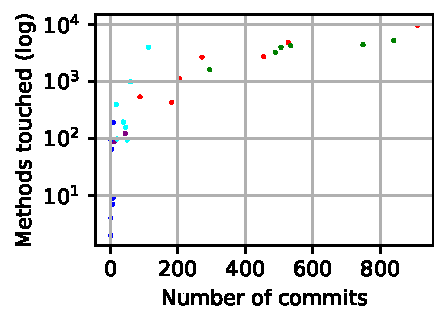
\includegraphics{sections/results/21/methods/sample_scatter_touched_against_commit.methods.sample.first.pdf}
    \caption{methods}
    \label{figure.sections/results/21/methods/sample_scatter_touched_against_commit.methods.sample.first.pdf}
  \end{subfigure}
\caption[Short]{\begin{minipage}[t]{\linewidth}Scatter plots of the log total number of components touched (y-axis) against the number of commits (x-axis) made by samples of developers capped at 84 sustained later joiners from six (6) categories: \color{Blue}Transient Founder (Blue, NUM1), \color{Purple}Moderate Founder (Purple, 3), \color{Green} Sustained Founder (Green, 7), \color{Orange} Transient Later Joiner (Orange, 84), \color{Cyan}Moderate Later Joiner (Cyan, 84), \color{Red} Sustained Later Joiner (Red, 84). \color{Black}\end{minipage}} 
\end{figure}
\clearpage 
\section{Sample scatter touched against commit - Repository: 21} 
\begin{figure}
  \centering 
  \begin{subfigure}[b] 
{0.45\textwidth}
    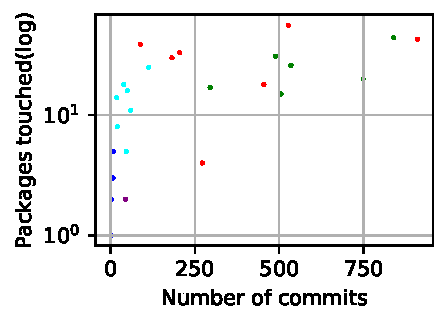
\includegraphics{sections/results/21/packages/sample_scatter_touched_against_commit.packages.sample.first.pdf}
    \caption{packages}
    \label{figure.sections/results/21/packages/sample_scatter_touched_against_commit.packages.sample.first.pdf}
  \end{subfigure}
\vspace{3mm}
  \begin{subfigure}[b] 
{0.45\textwidth}
    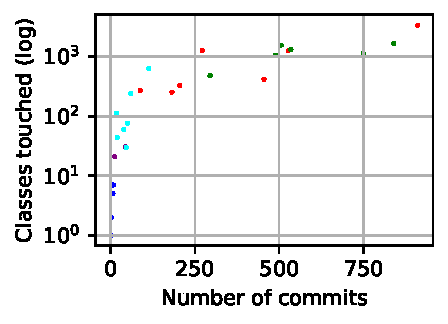
\includegraphics{sections/results/21/classes/sample_scatter_touched_against_commit.classes.sample.first.pdf}
    \caption{classes}
    \label{figure.sections/results/21/classes/sample_scatter_touched_against_commit.classes.sample.first.pdf}
  \end{subfigure}
  \begin{subfigure}[b] 
{0.45\textwidth}
    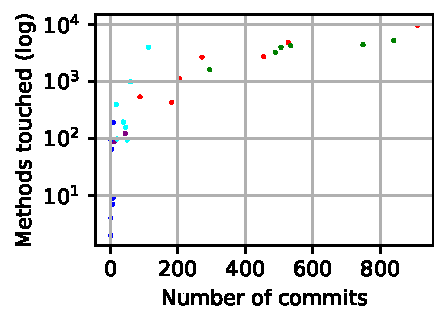
\includegraphics{sections/results/21/methods/sample_scatter_touched_against_commit.methods.sample.first.pdf}
    \caption{methods}
    \label{figure.sections/results/21/methods/sample_scatter_touched_against_commit.methods.sample.first.pdf}
  \end{subfigure}
\caption[Short]{\begin{minipage}[t]{\linewidth}Scatter plots of the log total number of components touched (y-axis) against the number of commits (x-axis) made by samples of developers capped at 84 sustained later joiners from six (6) categories: \color{Blue}Transient Founder (Blue, NUM1), \color{Purple}Moderate Founder (Purple, 3), \color{Green} Sustained Founder (Green, 7), \color{Orange} Transient Later Joiner (Orange, 84), \color{Cyan}Moderate Later Joiner (Cyan, 84), \color{Red} Sustained Later Joiner (Red, 84). \color{Black}\end{minipage}} 
\end{figure}
\clearpage 
\section{Sample scatter touched against commit - Repository: 21} 
\begin{figure}
  \centering 
  \begin{subfigure}[b] 
{0.45\textwidth}
    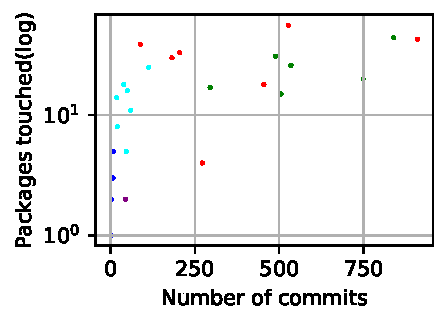
\includegraphics{sections/results/21/packages/sample_scatter_touched_against_commit.packages.sample.first.pdf}
    \caption{packages}
    \label{figure.sections/results/21/packages/sample_scatter_touched_against_commit.packages.sample.first.pdf}
  \end{subfigure}
\vspace{3mm}
  \begin{subfigure}[b] 
{0.45\textwidth}
    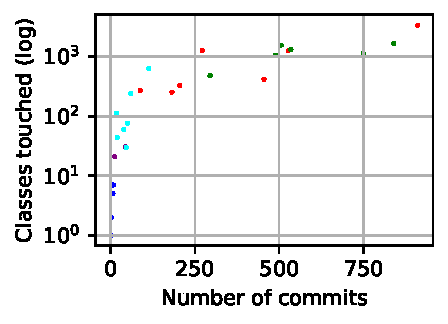
\includegraphics{sections/results/21/classes/sample_scatter_touched_against_commit.classes.sample.first.pdf}
    \caption{classes}
    \label{figure.sections/results/21/classes/sample_scatter_touched_against_commit.classes.sample.first.pdf}
  \end{subfigure}
  \begin{subfigure}[b] 
{0.45\textwidth}
    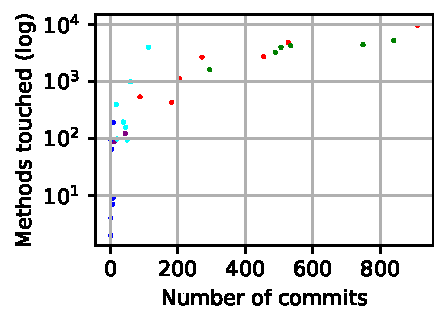
\includegraphics{sections/results/21/methods/sample_scatter_touched_against_commit.methods.sample.first.pdf}
    \caption{methods}
    \label{figure.sections/results/21/methods/sample_scatter_touched_against_commit.methods.sample.first.pdf}
  \end{subfigure}
\caption[Short]{\begin{minipage}[t]{\linewidth}Scatter plots of the log total number of components touched (y-axis) against the number of commits (x-axis) made by samples of developers capped at 84 sustained later joiners from six (6) categories: \color{Blue}Transient Founder (Blue, NUM1), \color{Purple}Moderate Founder (Purple, 3), \color{Green} Sustained Founder (Green, 7), \color{Orange} Transient Later Joiner (Orange, 84), \color{Cyan}Moderate Later Joiner (Cyan, 84), \color{Red} Sustained Later Joiner (Red, 84). \color{Black}\end{minipage}} 
\end{figure}
\clearpage 
\section{Sample scatter touched against commit - Repository: 21} 
\begin{figure}
  \centering 
  \begin{subfigure}[b] 
{0.45\textwidth}
    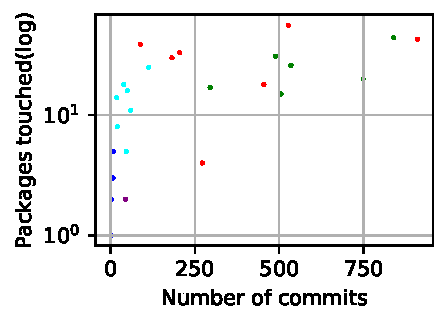
\includegraphics{sections/results/21/packages/sample_scatter_touched_against_commit.packages.sample.first.pdf}
    \caption{packages}
    \label{figure.sections/results/21/packages/sample_scatter_touched_against_commit.packages.sample.first.pdf}
  \end{subfigure}
\vspace{3mm}
  \begin{subfigure}[b] 
{0.45\textwidth}
    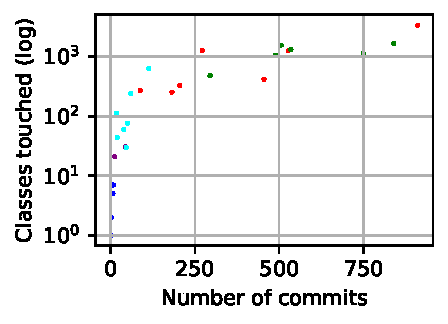
\includegraphics{sections/results/21/classes/sample_scatter_touched_against_commit.classes.sample.first.pdf}
    \caption{classes}
    \label{figure.sections/results/21/classes/sample_scatter_touched_against_commit.classes.sample.first.pdf}
  \end{subfigure}
  \begin{subfigure}[b] 
{0.45\textwidth}
    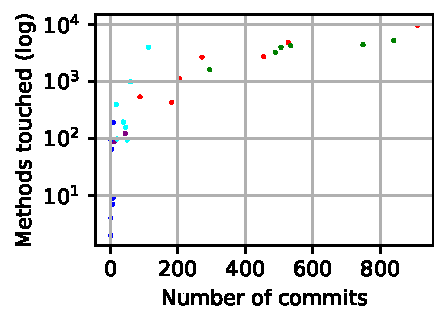
\includegraphics{sections/results/21/methods/sample_scatter_touched_against_commit.methods.sample.first.pdf}
    \caption{methods}
    \label{figure.sections/results/21/methods/sample_scatter_touched_against_commit.methods.sample.first.pdf}
  \end{subfigure}
\caption[Short]{\begin{minipage}[t]{\linewidth}Scatter plots of the log total number of components touched (y-axis) against the number of commits (x-axis) made by samples of developers capped at 84 sustained later joiners from six (6) categories: \color{Blue}Transient Founder (Blue, NUM1), \color{Purple}Moderate Founder (Purple, 3), \color{Green} Sustained Founder (Green, 7), \color{Orange} Transient Later Joiner (Orange, 84), \color{Cyan}Moderate Later Joiner (Cyan, 84), \color{Red} Sustained Later Joiner (Red, 84). \color{Black}\end{minipage}} 
\end{figure}
\clearpage 
\section{Sample scatter touched against commit - Repository: 21} 
\begin{figure}
  \centering 
  \begin{subfigure}[b] 
{0.45\textwidth}
    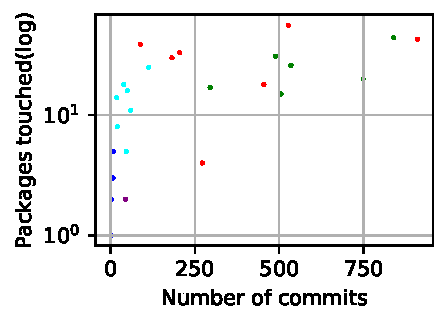
\includegraphics{sections/results/21/packages/sample_scatter_touched_against_commit.packages.sample.first.pdf}
    \caption{packages}
    \label{figure.sections/results/21/packages/sample_scatter_touched_against_commit.packages.sample.first.pdf}
  \end{subfigure}
\vspace{3mm}
  \begin{subfigure}[b] 
{0.45\textwidth}
    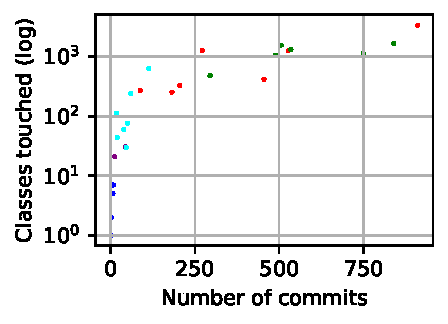
\includegraphics{sections/results/21/classes/sample_scatter_touched_against_commit.classes.sample.first.pdf}
    \caption{classes}
    \label{figure.sections/results/21/classes/sample_scatter_touched_against_commit.classes.sample.first.pdf}
  \end{subfigure}
  \begin{subfigure}[b] 
{0.45\textwidth}
    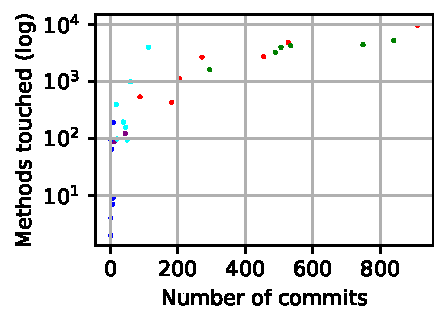
\includegraphics{sections/results/21/methods/sample_scatter_touched_against_commit.methods.sample.first.pdf}
    \caption{methods}
    \label{figure.sections/results/21/methods/sample_scatter_touched_against_commit.methods.sample.first.pdf}
  \end{subfigure}
\caption[Short]{\begin{minipage}[t]{\linewidth}Scatter plots of the log total number of components touched (y-axis) against the number of commits (x-axis) made by samples of developers capped at 84 sustained later joiners from six (6) categories: \color{Blue}Transient Founder (Blue, NUM1), \color{Purple}Moderate Founder (Purple, 3), \color{Green} Sustained Founder (Green, 7), \color{Orange} Transient Later Joiner (Orange, 84), \color{Cyan}Moderate Later Joiner (Cyan, 84), \color{Red} Sustained Later Joiner (Red, 84). \color{Black}\end{minipage}} 
\end{figure}
\clearpage 
\section{Sample scatter touched against commit - Repository: 21} 
\begin{figure}
  \centering 
  \begin{subfigure}[b] 
{0.45\textwidth}
    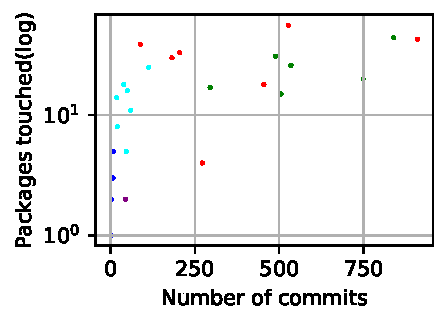
\includegraphics{sections/results/21/packages/sample_scatter_touched_against_commit.packages.sample.first.pdf}
    \caption{packages}
    \label{figure.sections/results/21/packages/sample_scatter_touched_against_commit.packages.sample.first.pdf}
  \end{subfigure}
\vspace{3mm}
  \begin{subfigure}[b] 
{0.45\textwidth}
    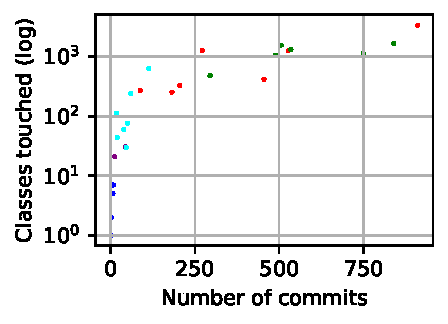
\includegraphics{sections/results/21/classes/sample_scatter_touched_against_commit.classes.sample.first.pdf}
    \caption{classes}
    \label{figure.sections/results/21/classes/sample_scatter_touched_against_commit.classes.sample.first.pdf}
  \end{subfigure}
  \begin{subfigure}[b] 
{0.45\textwidth}
    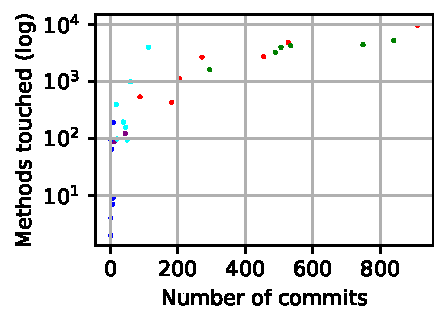
\includegraphics{sections/results/21/methods/sample_scatter_touched_against_commit.methods.sample.first.pdf}
    \caption{methods}
    \label{figure.sections/results/21/methods/sample_scatter_touched_against_commit.methods.sample.first.pdf}
  \end{subfigure}
\caption[Short]{\begin{minipage}[t]{\linewidth}Scatter plots of the log total number of components touched (y-axis) against the number of commits (x-axis) made by samples of developers capped at 84 sustained later joiners from six (6) categories: \color{Blue}Transient Founder (Blue, NUM1), \color{Purple}Moderate Founder (Purple, 3), \color{Green} Sustained Founder (Green, 7), \color{Orange} Transient Later Joiner (Orange, 84), \color{Cyan}Moderate Later Joiner (Cyan, 84), \color{Red} Sustained Later Joiner (Red, 84). \color{Black}\end{minipage}} 
\end{figure}
\clearpage 
\section{Sample scatter touched against commit - Repository: 21} 
\begin{figure}
  \centering 
  \begin{subfigure}[b] 
{0.45\textwidth}
    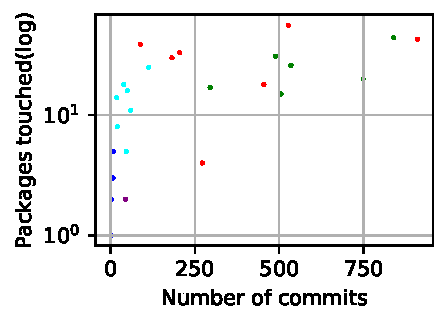
\includegraphics{sections/results/21/packages/sample_scatter_touched_against_commit.packages.sample.first.pdf}
    \caption{packages}
    \label{figure.sections/results/21/packages/sample_scatter_touched_against_commit.packages.sample.first.pdf}
  \end{subfigure}
\vspace{3mm}
  \begin{subfigure}[b] 
{0.45\textwidth}
    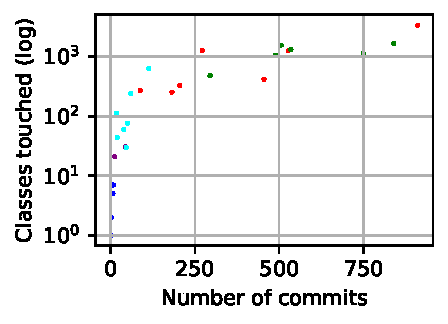
\includegraphics{sections/results/21/classes/sample_scatter_touched_against_commit.classes.sample.first.pdf}
    \caption{classes}
    \label{figure.sections/results/21/classes/sample_scatter_touched_against_commit.classes.sample.first.pdf}
  \end{subfigure}
  \begin{subfigure}[b] 
{0.45\textwidth}
    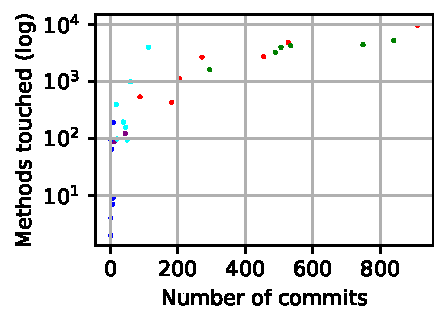
\includegraphics{sections/results/21/methods/sample_scatter_touched_against_commit.methods.sample.first.pdf}
    \caption{methods}
    \label{figure.sections/results/21/methods/sample_scatter_touched_against_commit.methods.sample.first.pdf}
  \end{subfigure}
\caption[Short]{\begin{minipage}[t]{\linewidth}Scatter plots of the log total number of components touched (y-axis) against the number of commits (x-axis) made by samples of developers capped at 84 sustained later joiners from six (6) categories: \color{Blue}Transient Founder (Blue, NUM1), \color{Purple}Moderate Founder (Purple, 3), \color{Green} Sustained Founder (Green, 7), \color{Orange} Transient Later Joiner (Orange, 84), \color{Cyan}Moderate Later Joiner (Cyan, 84), \color{Red} Sustained Later Joiner (Red, 84). \color{Black}\end{minipage}} 
\end{figure}
\clearpage 
\section{Sample scatter touched against commit - Repository: 21} 
\begin{figure}
  \centering 
  \begin{subfigure}[b] 
{0.45\textwidth}
    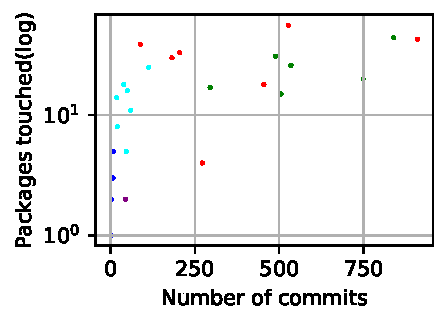
\includegraphics{sections/results/21/packages/sample_scatter_touched_against_commit.packages.sample.first.pdf}
    \caption{packages}
    \label{figure.sections/results/21/packages/sample_scatter_touched_against_commit.packages.sample.first.pdf}
  \end{subfigure}
\vspace{3mm}
  \begin{subfigure}[b] 
{0.45\textwidth}
    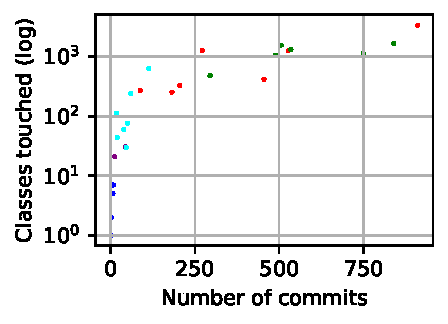
\includegraphics{sections/results/21/classes/sample_scatter_touched_against_commit.classes.sample.first.pdf}
    \caption{classes}
    \label{figure.sections/results/21/classes/sample_scatter_touched_against_commit.classes.sample.first.pdf}
  \end{subfigure}
  \begin{subfigure}[b] 
{0.45\textwidth}
    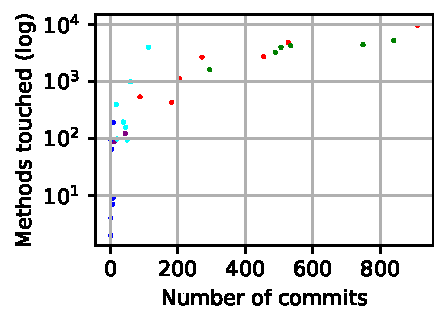
\includegraphics{sections/results/21/methods/sample_scatter_touched_against_commit.methods.sample.first.pdf}
    \caption{methods}
    \label{figure.sections/results/21/methods/sample_scatter_touched_against_commit.methods.sample.first.pdf}
  \end{subfigure}
\caption[Short]{\begin{minipage}[t]{\linewidth}Scatter plots of the log total number of components touched (y-axis) against the number of commits (x-axis) made by samples of developers capped at 84 sustained later joiners from six (6) categories: \color{Blue}Transient Founder (Blue, NUM1), \color{Purple}Moderate Founder (Purple, 3), \color{Green} Sustained Founder (Green, 7), \color{Orange} Transient Later Joiner (Orange, 84), \color{Cyan}Moderate Later Joiner (Cyan, 84), \color{Red} Sustained Later Joiner (Red, 84). \color{Black}\end{minipage}} 
\end{figure}
\clearpage 
\section{Sample scatter touched against commit - Repository: 21} 
\begin{figure}
  \centering 
  \begin{subfigure}[b] 
{0.45\textwidth}
    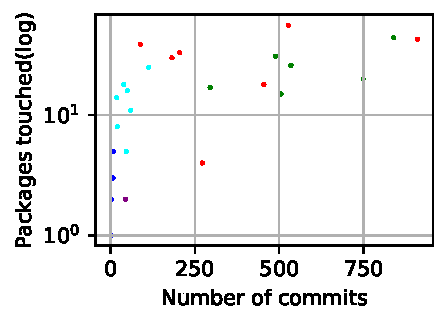
\includegraphics{sections/results/21/packages/sample_scatter_touched_against_commit.packages.sample.first.pdf}
    \caption{packages}
    \label{figure.sections/results/21/packages/sample_scatter_touched_against_commit.packages.sample.first.pdf}
  \end{subfigure}
\vspace{3mm}
  \begin{subfigure}[b] 
{0.45\textwidth}
    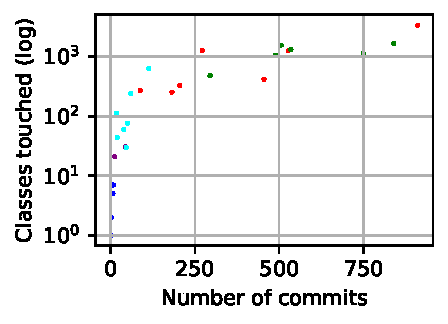
\includegraphics{sections/results/21/classes/sample_scatter_touched_against_commit.classes.sample.first.pdf}
    \caption{classes}
    \label{figure.sections/results/21/classes/sample_scatter_touched_against_commit.classes.sample.first.pdf}
  \end{subfigure}
  \begin{subfigure}[b] 
{0.45\textwidth}
    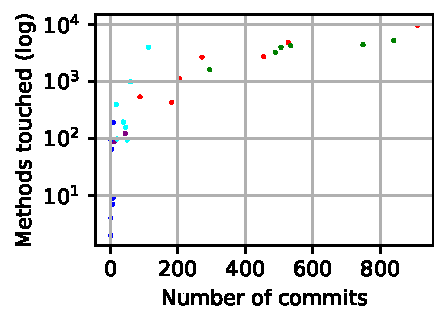
\includegraphics{sections/results/21/methods/sample_scatter_touched_against_commit.methods.sample.first.pdf}
    \caption{methods}
    \label{figure.sections/results/21/methods/sample_scatter_touched_against_commit.methods.sample.first.pdf}
  \end{subfigure}
\caption[Short]{\begin{minipage}[t]{\linewidth}Scatter plots of the log total number of components touched (y-axis) against the number of commits (x-axis) made by samples of developers capped at 84 sustained later joiners from six (6) categories: \color{Blue}Transient Founder (Blue, NUM1), \color{Purple}Moderate Founder (Purple, 3), \color{Green} Sustained Founder (Green, 7), \color{Orange} Transient Later Joiner (Orange, 84), \color{Cyan}Moderate Later Joiner (Cyan, 84), \color{Red} Sustained Later Joiner (Red, 84). \color{Black}\end{minipage}} 
\end{figure}
\clearpage 
\section{Sample scatter touched against commit - Repository: 21} 
\begin{figure}
  \centering 
  \begin{subfigure}[b] 
{0.45\textwidth}
    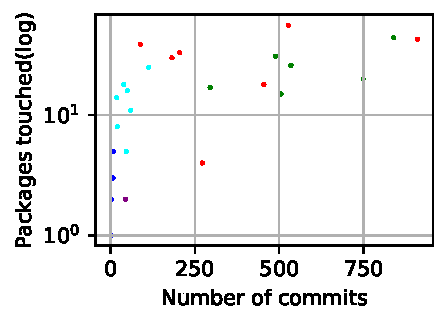
\includegraphics{sections/results/21/packages/sample_scatter_touched_against_commit.packages.sample.first.pdf}
    \caption{packages}
    \label{figure.sections/results/21/packages/sample_scatter_touched_against_commit.packages.sample.first.pdf}
  \end{subfigure}
\vspace{3mm}
  \begin{subfigure}[b] 
{0.45\textwidth}
    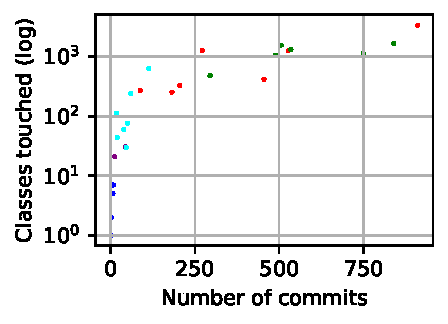
\includegraphics{sections/results/21/classes/sample_scatter_touched_against_commit.classes.sample.first.pdf}
    \caption{classes}
    \label{figure.sections/results/21/classes/sample_scatter_touched_against_commit.classes.sample.first.pdf}
  \end{subfigure}
  \begin{subfigure}[b] 
{0.45\textwidth}
    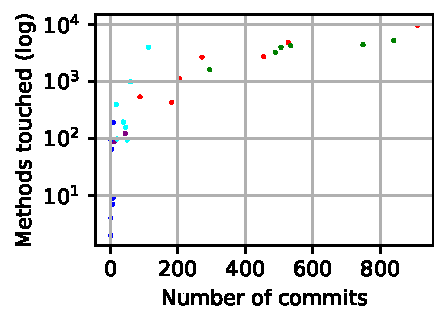
\includegraphics{sections/results/21/methods/sample_scatter_touched_against_commit.methods.sample.first.pdf}
    \caption{methods}
    \label{figure.sections/results/21/methods/sample_scatter_touched_against_commit.methods.sample.first.pdf}
  \end{subfigure}
\caption[Short]{\begin{minipage}[t]{\linewidth}Scatter plots of the log total number of components touched (y-axis) against the number of commits (x-axis) made by samples of developers capped at 84 sustained later joiners from six (6) categories: \color{Blue}Transient Founder (Blue, NUM1), \color{Purple}Moderate Founder (Purple, 3), \color{Green} Sustained Founder (Green, 7), \color{Orange} Transient Later Joiner (Orange, 84), \color{Cyan}Moderate Later Joiner (Cyan, 84), \color{Red} Sustained Later Joiner (Red, 84). \color{Black}\end{minipage}} 
\end{figure}
\clearpage 
\section{Sample scatter touched against commit - Repository: 21} 
\begin{figure}
  \centering 
  \begin{subfigure}[b] 
{0.45\textwidth}
    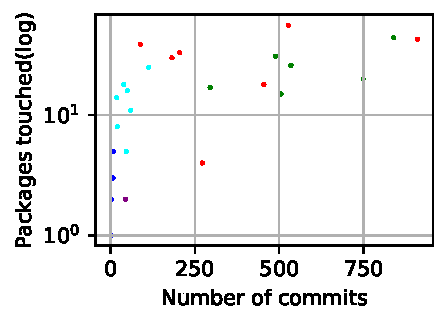
\includegraphics{sections/results/21/packages/sample_scatter_touched_against_commit.packages.sample.first.pdf}
    \caption{packages}
    \label{figure.sections/results/21/packages/sample_scatter_touched_against_commit.packages.sample.first.pdf}
  \end{subfigure}
\vspace{3mm}
  \begin{subfigure}[b] 
{0.45\textwidth}
    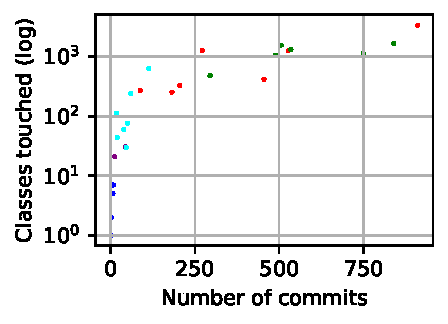
\includegraphics{sections/results/21/classes/sample_scatter_touched_against_commit.classes.sample.first.pdf}
    \caption{classes}
    \label{figure.sections/results/21/classes/sample_scatter_touched_against_commit.classes.sample.first.pdf}
  \end{subfigure}
  \begin{subfigure}[b] 
{0.45\textwidth}
    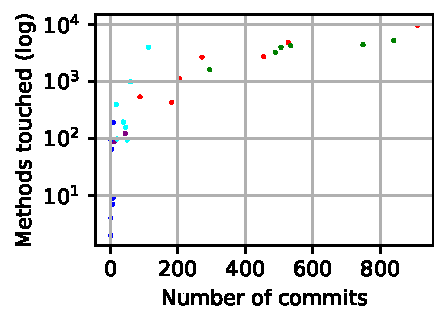
\includegraphics{sections/results/21/methods/sample_scatter_touched_against_commit.methods.sample.first.pdf}
    \caption{methods}
    \label{figure.sections/results/21/methods/sample_scatter_touched_against_commit.methods.sample.first.pdf}
  \end{subfigure}
\caption[Short]{\begin{minipage}[t]{\linewidth}Scatter plots of the log total number of components touched (y-axis) against the number of commits (x-axis) made by samples of developers capped at 84 sustained later joiners from six (6) categories: \color{Blue}Transient Founder (Blue, NUM1), \color{Purple}Moderate Founder (Purple, 3), \color{Green} Sustained Founder (Green, 7), \color{Orange} Transient Later Joiner (Orange, 84), \color{Cyan}Moderate Later Joiner (Cyan, 84), \color{Red} Sustained Later Joiner (Red, 84). \color{Black}\end{minipage}} 
\end{figure}
\clearpage 
\section{Sample scatter touched against commit - Repository: 21} 
\begin{figure}
  \centering 
  \begin{subfigure}[b] 
{0.45\textwidth}
    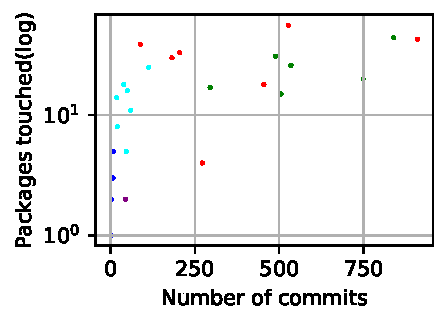
\includegraphics{sections/results/21/packages/sample_scatter_touched_against_commit.packages.sample.first.pdf}
    \caption{packages}
    \label{figure.sections/results/21/packages/sample_scatter_touched_against_commit.packages.sample.first.pdf}
  \end{subfigure}
\vspace{3mm}
  \begin{subfigure}[b] 
{0.45\textwidth}
    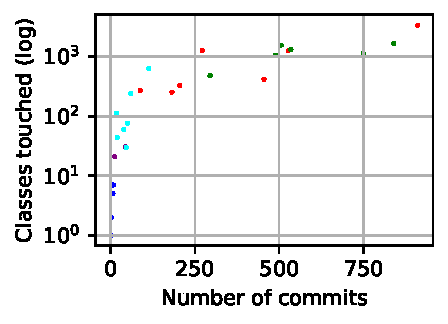
\includegraphics{sections/results/21/classes/sample_scatter_touched_against_commit.classes.sample.first.pdf}
    \caption{classes}
    \label{figure.sections/results/21/classes/sample_scatter_touched_against_commit.classes.sample.first.pdf}
  \end{subfigure}
  \begin{subfigure}[b] 
{0.45\textwidth}
    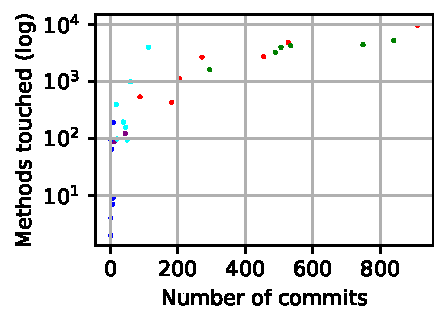
\includegraphics{sections/results/21/methods/sample_scatter_touched_against_commit.methods.sample.first.pdf}
    \caption{methods}
    \label{figure.sections/results/21/methods/sample_scatter_touched_against_commit.methods.sample.first.pdf}
  \end{subfigure}
\caption[Short]{\begin{minipage}[t]{\linewidth}Scatter plots of the log total number of components touched (y-axis) against the number of commits (x-axis) made by samples of developers capped at 84 sustained later joiners from six (6) categories: \color{Blue}Transient Founder (Blue, NUM1), \color{Purple}Moderate Founder (Purple, 3), \color{Green} Sustained Founder (Green, 7), \color{Orange} Transient Later Joiner (Orange, 84), \color{Cyan}Moderate Later Joiner (Cyan, 84), \color{Red} Sustained Later Joiner (Red, 84). \color{Black}\end{minipage}} 
\end{figure}
\clearpage 
\section{Sample scatter touched against commit - Repository: 21} 
\begin{figure}
  \centering 
  \begin{subfigure}[b] 
{0.45\textwidth}
    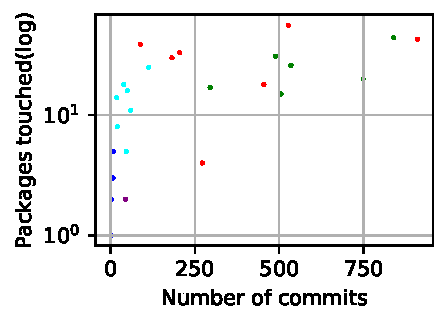
\includegraphics{sections/results/21/packages/sample_scatter_touched_against_commit.packages.sample.first.pdf}
    \caption{packages}
    \label{figure.sections/results/21/packages/sample_scatter_touched_against_commit.packages.sample.first.pdf}
  \end{subfigure}
\vspace{3mm}
  \begin{subfigure}[b] 
{0.45\textwidth}
    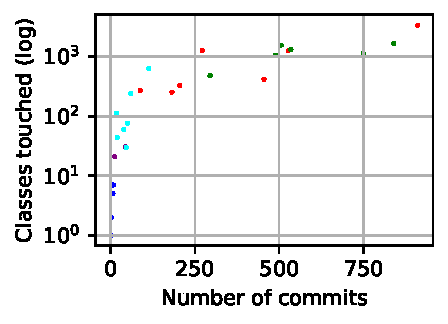
\includegraphics{sections/results/21/classes/sample_scatter_touched_against_commit.classes.sample.first.pdf}
    \caption{classes}
    \label{figure.sections/results/21/classes/sample_scatter_touched_against_commit.classes.sample.first.pdf}
  \end{subfigure}
  \begin{subfigure}[b] 
{0.45\textwidth}
    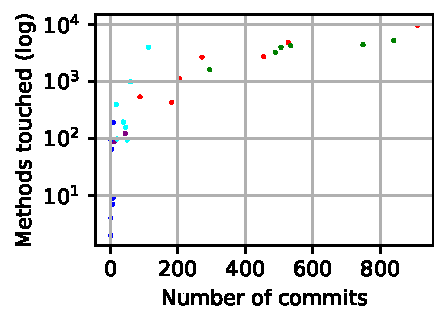
\includegraphics{sections/results/21/methods/sample_scatter_touched_against_commit.methods.sample.first.pdf}
    \caption{methods}
    \label{figure.sections/results/21/methods/sample_scatter_touched_against_commit.methods.sample.first.pdf}
  \end{subfigure}
\caption[Short]{\begin{minipage}[t]{\linewidth}Scatter plots of the log total number of components touched (y-axis) against the number of commits (x-axis) made by samples of developers capped at 84 sustained later joiners from six (6) categories: \color{Blue}Transient Founder (Blue, NUM1), \color{Purple}Moderate Founder (Purple, 3), \color{Green} Sustained Founder (Green, 7), \color{Orange} Transient Later Joiner (Orange, 84), \color{Cyan}Moderate Later Joiner (Cyan, 84), \color{Red} Sustained Later Joiner (Red, 84). \color{Black}\end{minipage}} 
\end{figure}
\clearpage 
\section{Sample scatter touched against commit - Repository: 21} 
\begin{figure}
  \centering 
  \begin{subfigure}[b] 
{0.45\textwidth}
    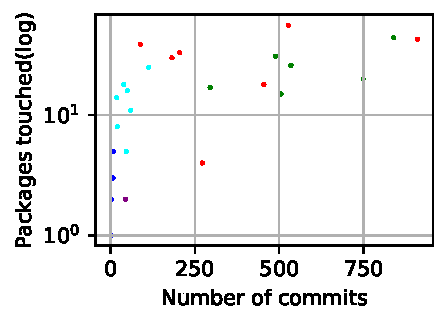
\includegraphics{sections/results/21/packages/sample_scatter_touched_against_commit.packages.sample.first.pdf}
    \caption{packages}
    \label{figure.sections/results/21/packages/sample_scatter_touched_against_commit.packages.sample.first.pdf}
  \end{subfigure}
\vspace{3mm}
  \begin{subfigure}[b] 
{0.45\textwidth}
    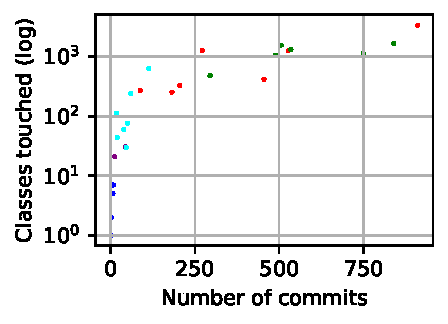
\includegraphics{sections/results/21/classes/sample_scatter_touched_against_commit.classes.sample.first.pdf}
    \caption{classes}
    \label{figure.sections/results/21/classes/sample_scatter_touched_against_commit.classes.sample.first.pdf}
  \end{subfigure}
  \begin{subfigure}[b] 
{0.45\textwidth}
    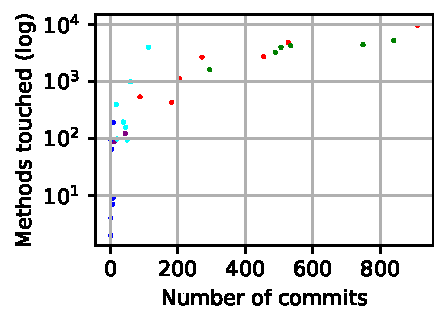
\includegraphics{sections/results/21/methods/sample_scatter_touched_against_commit.methods.sample.first.pdf}
    \caption{methods}
    \label{figure.sections/results/21/methods/sample_scatter_touched_against_commit.methods.sample.first.pdf}
  \end{subfigure}
\caption[Short]{\begin{minipage}[t]{\linewidth}Scatter plots of the log total number of components touched (y-axis) against the number of commits (x-axis) made by samples of developers capped at 84 sustained later joiners from six (6) categories: \color{Blue}Transient Founder (Blue, NUM1), \color{Purple}Moderate Founder (Purple, 3), \color{Green} Sustained Founder (Green, 7), \color{Orange} Transient Later Joiner (Orange, 84), \color{Cyan}Moderate Later Joiner (Cyan, 84), \color{Red} Sustained Later Joiner (Red, 84). \color{Black}\end{minipage}} 
\end{figure}
\clearpage 
\section{Sample scatter touched against commit - Repository: 21} 
\begin{figure}
  \centering 
  \begin{subfigure}[b] 
{0.45\textwidth}
    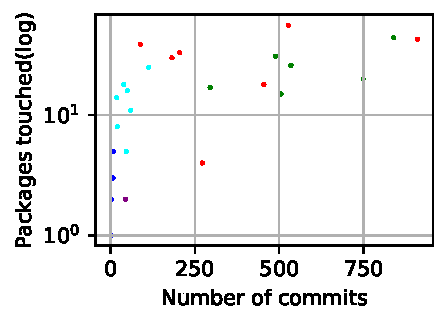
\includegraphics{sections/results/21/packages/sample_scatter_touched_against_commit.packages.sample.first.pdf}
    \caption{packages}
    \label{figure.sections/results/21/packages/sample_scatter_touched_against_commit.packages.sample.first.pdf}
  \end{subfigure}
\vspace{3mm}
  \begin{subfigure}[b] 
{0.45\textwidth}
    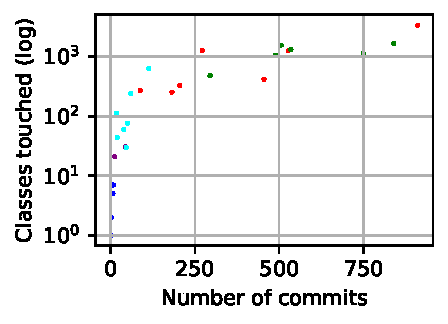
\includegraphics{sections/results/21/classes/sample_scatter_touched_against_commit.classes.sample.first.pdf}
    \caption{classes}
    \label{figure.sections/results/21/classes/sample_scatter_touched_against_commit.classes.sample.first.pdf}
  \end{subfigure}
  \begin{subfigure}[b] 
{0.45\textwidth}
    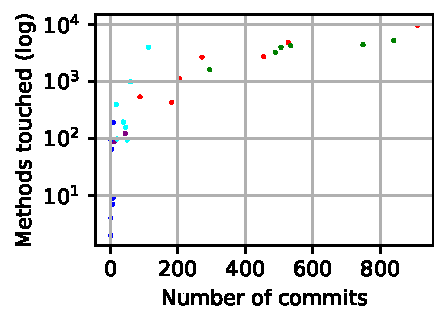
\includegraphics{sections/results/21/methods/sample_scatter_touched_against_commit.methods.sample.first.pdf}
    \caption{methods}
    \label{figure.sections/results/21/methods/sample_scatter_touched_against_commit.methods.sample.first.pdf}
  \end{subfigure}
\caption[Short]{\begin{minipage}[t]{\linewidth}Scatter plots of the log total number of components touched (y-axis) against the number of commits (x-axis) made by samples of developers capped at 84 sustained later joiners from six (6) categories: \color{Blue}Transient Founder (Blue, NUM1), \color{Purple}Moderate Founder (Purple, 3), \color{Green} Sustained Founder (Green, 7), \color{Orange} Transient Later Joiner (Orange, 84), \color{Cyan}Moderate Later Joiner (Cyan, 84), \color{Red} Sustained Later Joiner (Red, 84). \color{Black}\end{minipage}} 
\end{figure}
\clearpage 
\section{Sample scatter touched against commit - Repository: 21} 
\begin{figure}
  \centering 
  \begin{subfigure}[b] 
{0.45\textwidth}
    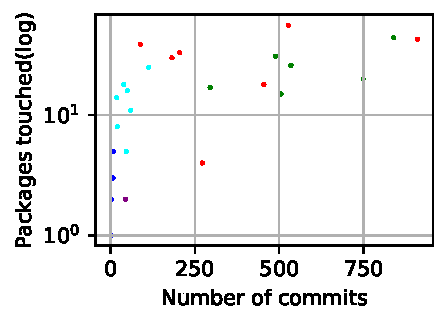
\includegraphics{sections/results/21/packages/sample_scatter_touched_against_commit.packages.sample.first.pdf}
    \caption{packages}
    \label{figure.sections/results/21/packages/sample_scatter_touched_against_commit.packages.sample.first.pdf}
  \end{subfigure}
\vspace{3mm}
  \begin{subfigure}[b] 
{0.45\textwidth}
    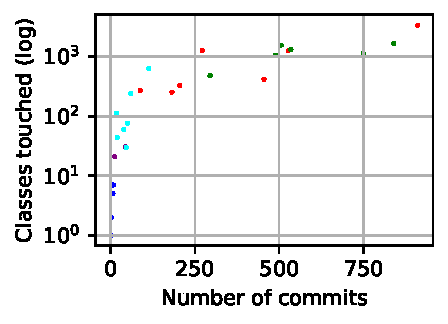
\includegraphics{sections/results/21/classes/sample_scatter_touched_against_commit.classes.sample.first.pdf}
    \caption{classes}
    \label{figure.sections/results/21/classes/sample_scatter_touched_against_commit.classes.sample.first.pdf}
  \end{subfigure}
  \begin{subfigure}[b] 
{0.45\textwidth}
    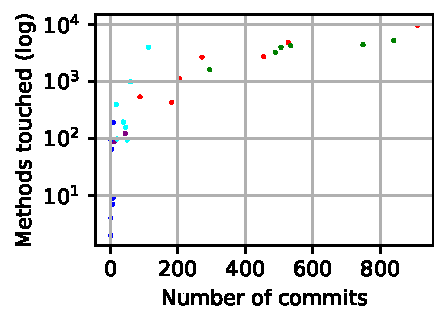
\includegraphics{sections/results/21/methods/sample_scatter_touched_against_commit.methods.sample.first.pdf}
    \caption{methods}
    \label{figure.sections/results/21/methods/sample_scatter_touched_against_commit.methods.sample.first.pdf}
  \end{subfigure}
\caption[Short]{\begin{minipage}[t]{\linewidth}Scatter plots of the log total number of components touched (y-axis) against the number of commits (x-axis) made by samples of developers capped at 84 sustained later joiners from six (6) categories: \color{Blue}Transient Founder (Blue, NUM1), \color{Purple}Moderate Founder (Purple, 3), \color{Green} Sustained Founder (Green, 7), \color{Orange} Transient Later Joiner (Orange, 84), \color{Cyan}Moderate Later Joiner (Cyan, 84), \color{Red} Sustained Later Joiner (Red, 84). \color{Black}\end{minipage}} 
\end{figure}
\clearpage 
\section{Sample scatter touched against commit - Repository: 21} 
\begin{figure}
  \centering 
  \begin{subfigure}[b] 
{0.45\textwidth}
    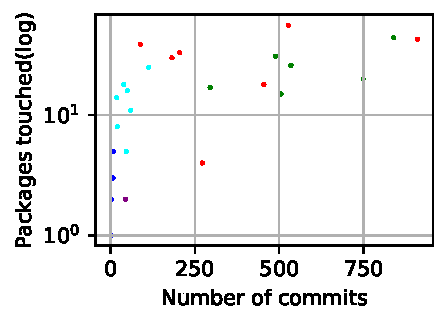
\includegraphics{sections/results/21/packages/sample_scatter_touched_against_commit.packages.sample.first.pdf}
    \caption{packages}
    \label{figure.sections/results/21/packages/sample_scatter_touched_against_commit.packages.sample.first.pdf}
  \end{subfigure}
\vspace{3mm}
  \begin{subfigure}[b] 
{0.45\textwidth}
    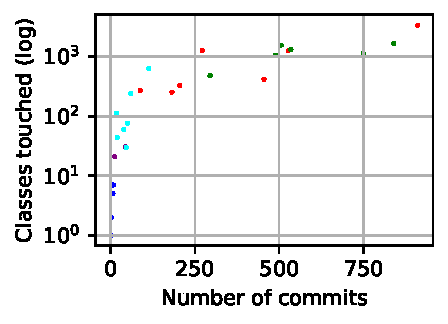
\includegraphics{sections/results/21/classes/sample_scatter_touched_against_commit.classes.sample.first.pdf}
    \caption{classes}
    \label{figure.sections/results/21/classes/sample_scatter_touched_against_commit.classes.sample.first.pdf}
  \end{subfigure}
  \begin{subfigure}[b] 
{0.45\textwidth}
    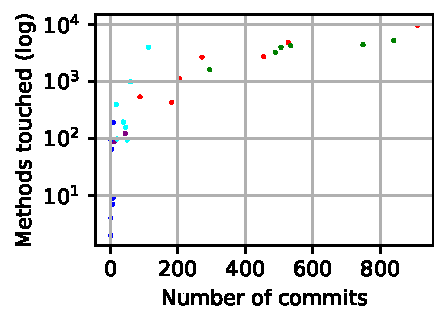
\includegraphics{sections/results/21/methods/sample_scatter_touched_against_commit.methods.sample.first.pdf}
    \caption{methods}
    \label{figure.sections/results/21/methods/sample_scatter_touched_against_commit.methods.sample.first.pdf}
  \end{subfigure}
\caption[Short]{\begin{minipage}[t]{\linewidth}Scatter plots of the log total number of components touched (y-axis) against the number of commits (x-axis) made by samples of developers capped at 84 sustained later joiners from six (6) categories: \color{Blue}Transient Founder (Blue, NUM1), \color{Purple}Moderate Founder (Purple, 3), \color{Green} Sustained Founder (Green, 7), \color{Orange} Transient Later Joiner (Orange, 84), \color{Cyan}Moderate Later Joiner (Cyan, 84), \color{Red} Sustained Later Joiner (Red, 84). \color{Black}\end{minipage}} 
\end{figure}
\clearpage 
\section{Sample scatter touched against commit - Repository: 21} 
\begin{figure}
  \centering 
  \begin{subfigure}[b] 
{0.45\textwidth}
    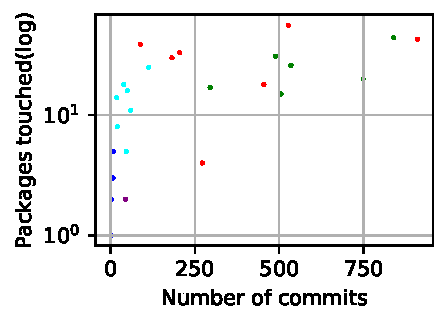
\includegraphics{sections/results/21/packages/sample_scatter_touched_against_commit.packages.sample.first.pdf}
    \caption{packages}
    \label{figure.sections/results/21/packages/sample_scatter_touched_against_commit.packages.sample.first.pdf}
  \end{subfigure}
\vspace{3mm}
  \begin{subfigure}[b] 
{0.45\textwidth}
    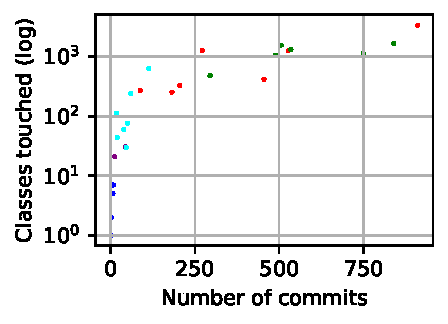
\includegraphics{sections/results/21/classes/sample_scatter_touched_against_commit.classes.sample.first.pdf}
    \caption{classes}
    \label{figure.sections/results/21/classes/sample_scatter_touched_against_commit.classes.sample.first.pdf}
  \end{subfigure}
  \begin{subfigure}[b] 
{0.45\textwidth}
    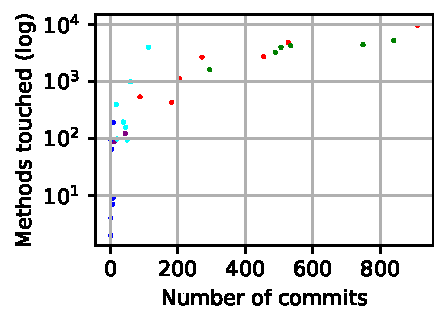
\includegraphics{sections/results/21/methods/sample_scatter_touched_against_commit.methods.sample.first.pdf}
    \caption{methods}
    \label{figure.sections/results/21/methods/sample_scatter_touched_against_commit.methods.sample.first.pdf}
  \end{subfigure}
\caption[Short]{\begin{minipage}[t]{\linewidth}Scatter plots of the log total number of components touched (y-axis) against the number of commits (x-axis) made by samples of developers capped at 84 sustained later joiners from six (6) categories: \color{Blue}Transient Founder (Blue, NUM1), \color{Purple}Moderate Founder (Purple, 3), \color{Green} Sustained Founder (Green, 7), \color{Orange} Transient Later Joiner (Orange, 84), \color{Cyan}Moderate Later Joiner (Cyan, 84), \color{Red} Sustained Later Joiner (Red, 84). \color{Black}\end{minipage}} 
\end{figure}
\clearpage 
\section{Sample scatter touched against commit - Repository: 21} 
\begin{figure}
  \centering 
  \begin{subfigure}[b] 
{0.45\textwidth}
    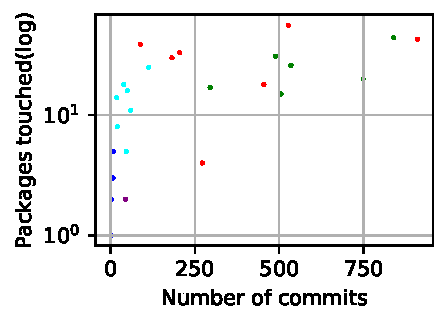
\includegraphics{sections/results/21/packages/sample_scatter_touched_against_commit.packages.sample.first.pdf}
    \caption{packages}
    \label{figure.sections/results/21/packages/sample_scatter_touched_against_commit.packages.sample.first.pdf}
  \end{subfigure}
\vspace{3mm}
  \begin{subfigure}[b] 
{0.45\textwidth}
    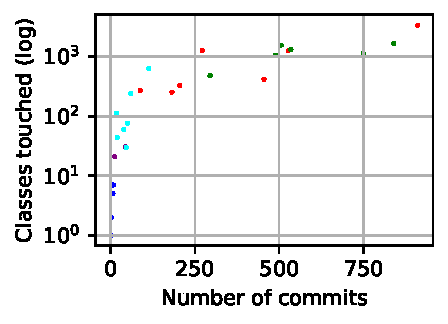
\includegraphics{sections/results/21/classes/sample_scatter_touched_against_commit.classes.sample.first.pdf}
    \caption{classes}
    \label{figure.sections/results/21/classes/sample_scatter_touched_against_commit.classes.sample.first.pdf}
  \end{subfigure}
  \begin{subfigure}[b] 
{0.45\textwidth}
    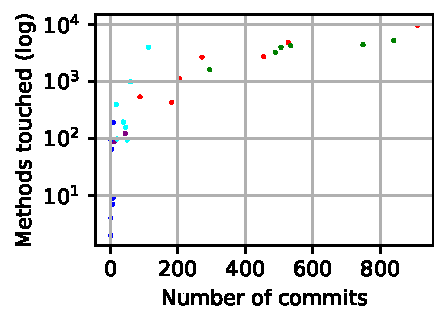
\includegraphics{sections/results/21/methods/sample_scatter_touched_against_commit.methods.sample.first.pdf}
    \caption{methods}
    \label{figure.sections/results/21/methods/sample_scatter_touched_against_commit.methods.sample.first.pdf}
  \end{subfigure}
\caption[Short]{\begin{minipage}[t]{\linewidth}Scatter plots of the log total number of components touched (y-axis) against the number of commits (x-axis) made by samples of developers capped at 84 sustained later joiners from six (6) categories: \color{Blue}Transient Founder (Blue, NUM1), \color{Purple}Moderate Founder (Purple, 3), \color{Green} Sustained Founder (Green, 7), \color{Orange} Transient Later Joiner (Orange, 84), \color{Cyan}Moderate Later Joiner (Cyan, 84), \color{Red} Sustained Later Joiner (Red, 84). \color{Black}\end{minipage}} 
\end{figure}
\clearpage 
\section{Sample scatter touched against commit - Repository: 21} 
\begin{figure}
  \centering 
  \begin{subfigure}[b] 
{0.45\textwidth}
    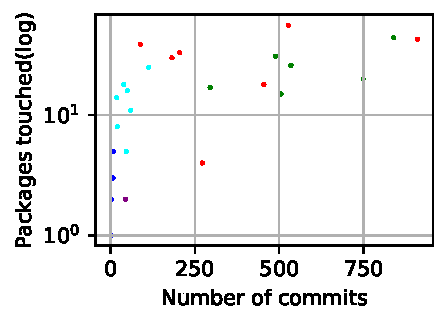
\includegraphics{sections/results/21/packages/sample_scatter_touched_against_commit.packages.sample.first.pdf}
    \caption{packages}
    \label{figure.sections/results/21/packages/sample_scatter_touched_against_commit.packages.sample.first.pdf}
  \end{subfigure}
\vspace{3mm}
  \begin{subfigure}[b] 
{0.45\textwidth}
    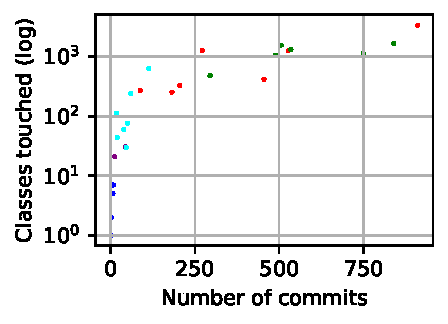
\includegraphics{sections/results/21/classes/sample_scatter_touched_against_commit.classes.sample.first.pdf}
    \caption{classes}
    \label{figure.sections/results/21/classes/sample_scatter_touched_against_commit.classes.sample.first.pdf}
  \end{subfigure}
  \begin{subfigure}[b] 
{0.45\textwidth}
    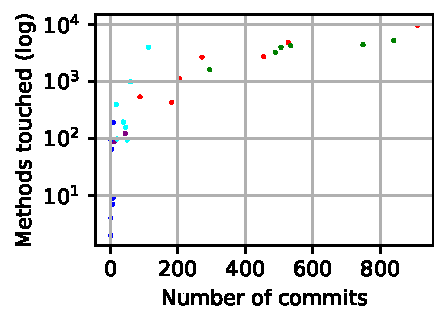
\includegraphics{sections/results/21/methods/sample_scatter_touched_against_commit.methods.sample.first.pdf}
    \caption{methods}
    \label{figure.sections/results/21/methods/sample_scatter_touched_against_commit.methods.sample.first.pdf}
  \end{subfigure}
\caption[Short]{\begin{minipage}[t]{\linewidth}Scatter plots of the log total number of components touched (y-axis) against the number of commits (x-axis) made by samples of developers capped at 84 sustained later joiners from six (6) categories: \color{Blue}Transient Founder (Blue, NUM1), \color{Purple}Moderate Founder (Purple, 3), \color{Green} Sustained Founder (Green, 7), \color{Orange} Transient Later Joiner (Orange, 84), \color{Cyan}Moderate Later Joiner (Cyan, 84), \color{Red} Sustained Later Joiner (Red, 84). \color{Black}\end{minipage}} 
\end{figure}
\clearpage 
\section{Sample scatter touched against commit - Repository: 21} 
\begin{figure}
  \centering 
  \begin{subfigure}[b] 
{0.45\textwidth}
    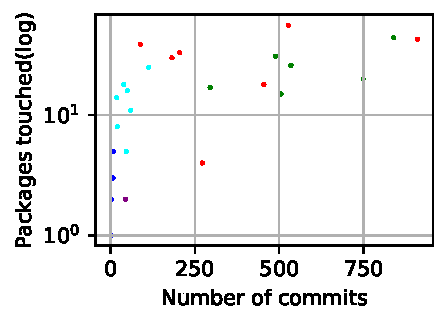
\includegraphics{sections/results/21/packages/sample_scatter_touched_against_commit.packages.sample.first.pdf}
    \caption{packages}
    \label{figure.sections/results/21/packages/sample_scatter_touched_against_commit.packages.sample.first.pdf}
  \end{subfigure}
\vspace{3mm}
  \begin{subfigure}[b] 
{0.45\textwidth}
    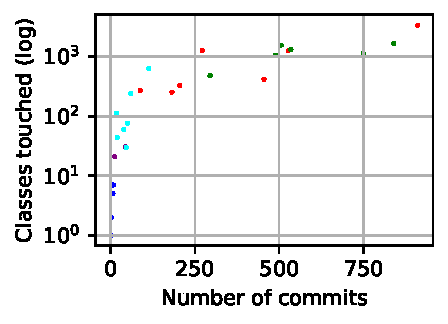
\includegraphics{sections/results/21/classes/sample_scatter_touched_against_commit.classes.sample.first.pdf}
    \caption{classes}
    \label{figure.sections/results/21/classes/sample_scatter_touched_against_commit.classes.sample.first.pdf}
  \end{subfigure}
  \begin{subfigure}[b] 
{0.45\textwidth}
    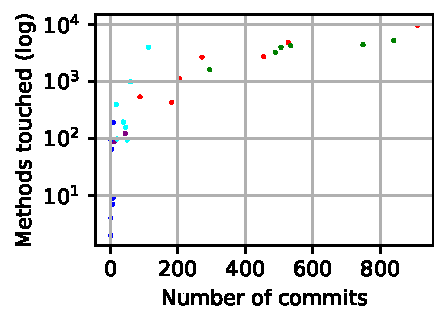
\includegraphics{sections/results/21/methods/sample_scatter_touched_against_commit.methods.sample.first.pdf}
    \caption{methods}
    \label{figure.sections/results/21/methods/sample_scatter_touched_against_commit.methods.sample.first.pdf}
  \end{subfigure}
\caption[Short]{\begin{minipage}[t]{\linewidth}Scatter plots of the log total number of components touched (y-axis) against the number of commits (x-axis) made by samples of developers capped at 84 sustained later joiners from six (6) categories: \color{Blue}Transient Founder (Blue, NUM1), \color{Purple}Moderate Founder (Purple, 3), \color{Green} Sustained Founder (Green, 7), \color{Orange} Transient Later Joiner (Orange, 84), \color{Cyan}Moderate Later Joiner (Cyan, 84), \color{Red} Sustained Later Joiner (Red, 84). \color{Black}\end{minipage}} 
\end{figure}
\clearpage 
\section{Sample scatter touched against commit - Repository: 21} 
\begin{figure}
  \centering 
  \begin{subfigure}[b] 
{0.45\textwidth}
    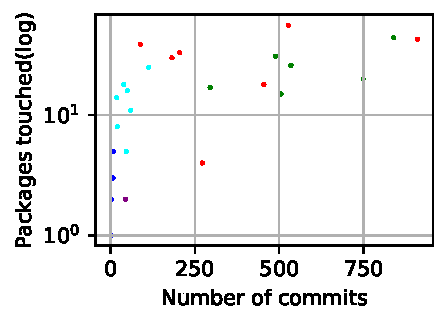
\includegraphics{sections/results/21/packages/sample_scatter_touched_against_commit.packages.sample.first.pdf}
    \caption{packages}
    \label{figure.sections/results/21/packages/sample_scatter_touched_against_commit.packages.sample.first.pdf}
  \end{subfigure}
\vspace{3mm}
  \begin{subfigure}[b] 
{0.45\textwidth}
    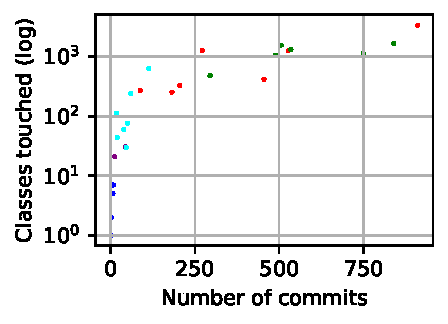
\includegraphics{sections/results/21/classes/sample_scatter_touched_against_commit.classes.sample.first.pdf}
    \caption{classes}
    \label{figure.sections/results/21/classes/sample_scatter_touched_against_commit.classes.sample.first.pdf}
  \end{subfigure}
  \begin{subfigure}[b] 
{0.45\textwidth}
    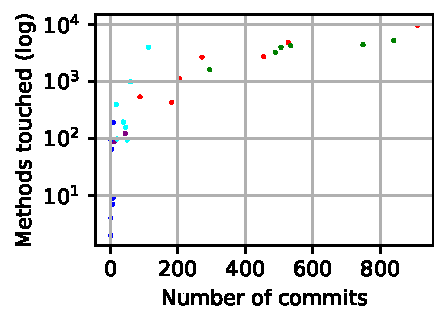
\includegraphics{sections/results/21/methods/sample_scatter_touched_against_commit.methods.sample.first.pdf}
    \caption{methods}
    \label{figure.sections/results/21/methods/sample_scatter_touched_against_commit.methods.sample.first.pdf}
  \end{subfigure}
\caption[Short]{\begin{minipage}[t]{\linewidth}Scatter plots of the log total number of components touched (y-axis) against the number of commits (x-axis) made by samples of developers capped at 84 sustained later joiners from six (6) categories: \color{Blue}Transient Founder (Blue, NUM1), \color{Purple}Moderate Founder (Purple, 3), \color{Green} Sustained Founder (Green, 7), \color{Orange} Transient Later Joiner (Orange, 84), \color{Cyan}Moderate Later Joiner (Cyan, 84), \color{Red} Sustained Later Joiner (Red, 84). \color{Black}\end{minipage}} 
\end{figure}
\clearpage 
\section{Sample scatter touched against commit - Repository: 21} 
\begin{figure}
  \centering 
  \begin{subfigure}[b] 
{0.45\textwidth}
    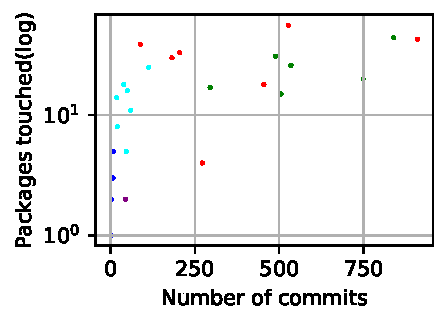
\includegraphics{sections/results/21/packages/sample_scatter_touched_against_commit.packages.sample.first.pdf}
    \caption{packages}
    \label{figure.sections/results/21/packages/sample_scatter_touched_against_commit.packages.sample.first.pdf}
  \end{subfigure}
\vspace{3mm}
  \begin{subfigure}[b] 
{0.45\textwidth}
    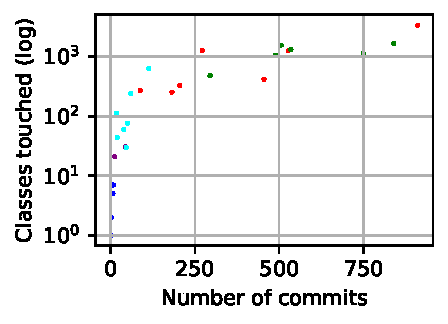
\includegraphics{sections/results/21/classes/sample_scatter_touched_against_commit.classes.sample.first.pdf}
    \caption{classes}
    \label{figure.sections/results/21/classes/sample_scatter_touched_against_commit.classes.sample.first.pdf}
  \end{subfigure}
  \begin{subfigure}[b] 
{0.45\textwidth}
    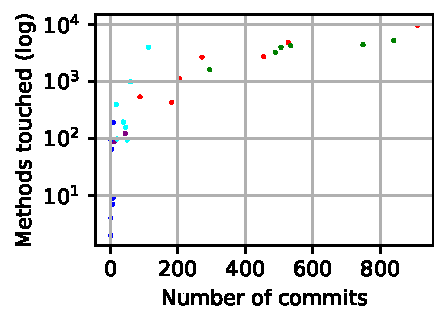
\includegraphics{sections/results/21/methods/sample_scatter_touched_against_commit.methods.sample.first.pdf}
    \caption{methods}
    \label{figure.sections/results/21/methods/sample_scatter_touched_against_commit.methods.sample.first.pdf}
  \end{subfigure}
\caption[Short]{\begin{minipage}[t]{\linewidth}Scatter plots of the log total number of components touched (y-axis) against the number of commits (x-axis) made by samples of developers capped at 84 sustained later joiners from six (6) categories: \color{Blue}Transient Founder (Blue, NUM1), \color{Purple}Moderate Founder (Purple, 3), \color{Green} Sustained Founder (Green, 7), \color{Orange} Transient Later Joiner (Orange, 84), \color{Cyan}Moderate Later Joiner (Cyan, 84), \color{Red} Sustained Later Joiner (Red, 84). \color{Black}\end{minipage}} 
\end{figure}
\clearpage 
\section{Sample scatter touched against commit - Repository: 21} 
\begin{figure}
  \centering 
  \begin{subfigure}[b] 
{0.45\textwidth}
    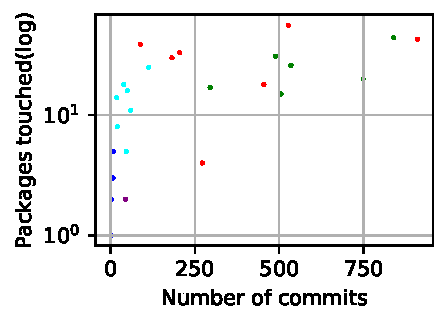
\includegraphics{sections/results/21/packages/sample_scatter_touched_against_commit.packages.sample.first.pdf}
    \caption{packages}
    \label{figure.sections/results/21/packages/sample_scatter_touched_against_commit.packages.sample.first.pdf}
  \end{subfigure}
\vspace{3mm}
  \begin{subfigure}[b] 
{0.45\textwidth}
    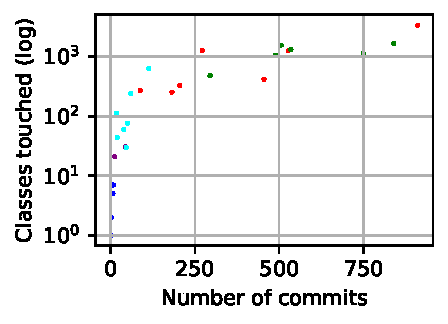
\includegraphics{sections/results/21/classes/sample_scatter_touched_against_commit.classes.sample.first.pdf}
    \caption{classes}
    \label{figure.sections/results/21/classes/sample_scatter_touched_against_commit.classes.sample.first.pdf}
  \end{subfigure}
  \begin{subfigure}[b] 
{0.45\textwidth}
    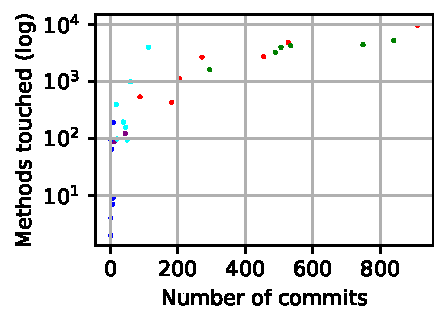
\includegraphics{sections/results/21/methods/sample_scatter_touched_against_commit.methods.sample.first.pdf}
    \caption{methods}
    \label{figure.sections/results/21/methods/sample_scatter_touched_against_commit.methods.sample.first.pdf}
  \end{subfigure}
\caption[Short]{\begin{minipage}[t]{\linewidth}Scatter plots of the log total number of components touched (y-axis) against the number of commits (x-axis) made by samples of developers capped at 84 sustained later joiners from six (6) categories: \color{Blue}Transient Founder (Blue, NUM1), \color{Purple}Moderate Founder (Purple, 3), \color{Green} Sustained Founder (Green, 7), \color{Orange} Transient Later Joiner (Orange, 84), \color{Cyan}Moderate Later Joiner (Cyan, 84), \color{Red} Sustained Later Joiner (Red, 84). \color{Black}\end{minipage}} 
\end{figure}
\clearpage 
\section{Sample scatter touched against commit - Repository: 21} 
\begin{figure}
  \centering 
  \begin{subfigure}[b] 
{0.45\textwidth}
    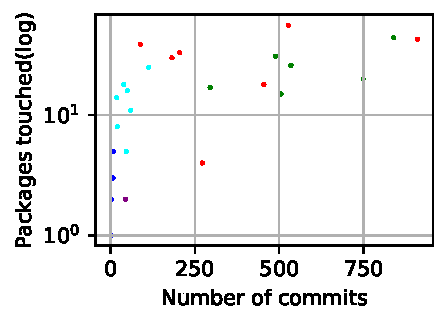
\includegraphics{sections/results/21/packages/sample_scatter_touched_against_commit.packages.sample.first.pdf}
    \caption{packages}
    \label{figure.sections/results/21/packages/sample_scatter_touched_against_commit.packages.sample.first.pdf}
  \end{subfigure}
\vspace{3mm}
  \begin{subfigure}[b] 
{0.45\textwidth}
    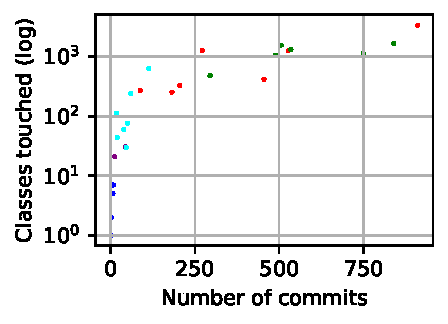
\includegraphics{sections/results/21/classes/sample_scatter_touched_against_commit.classes.sample.first.pdf}
    \caption{classes}
    \label{figure.sections/results/21/classes/sample_scatter_touched_against_commit.classes.sample.first.pdf}
  \end{subfigure}
  \begin{subfigure}[b] 
{0.45\textwidth}
    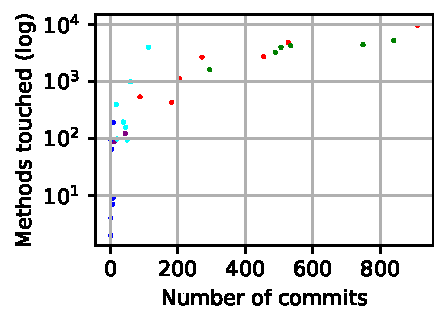
\includegraphics{sections/results/21/methods/sample_scatter_touched_against_commit.methods.sample.first.pdf}
    \caption{methods}
    \label{figure.sections/results/21/methods/sample_scatter_touched_against_commit.methods.sample.first.pdf}
  \end{subfigure}
\caption[Short]{\begin{minipage}[t]{\linewidth}Scatter plots of the log total number of components touched (y-axis) against the number of commits (x-axis) made by samples of developers capped at 84 sustained later joiners from six (6) categories: \color{Blue}Transient Founder (Blue, NUM1), \color{Purple}Moderate Founder (Purple, 3), \color{Green} Sustained Founder (Green, 7), \color{Orange} Transient Later Joiner (Orange, 84), \color{Cyan}Moderate Later Joiner (Cyan, 84), \color{Red} Sustained Later Joiner (Red, 84). \color{Black}\end{minipage}} 
\end{figure}
\clearpage 
\section{Sample scatter touched against commit - Repository: 21} 
\begin{figure}
  \centering 
  \begin{subfigure}[b] 
{0.45\textwidth}
    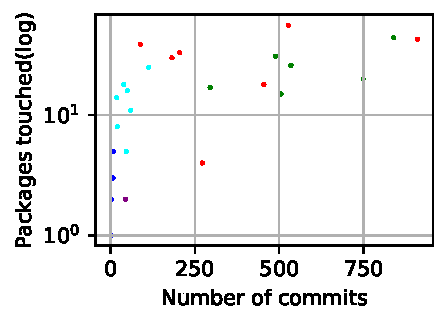
\includegraphics{sections/results/21/packages/sample_scatter_touched_against_commit.packages.sample.first.pdf}
    \caption{packages}
    \label{figure.sections/results/21/packages/sample_scatter_touched_against_commit.packages.sample.first.pdf}
  \end{subfigure}
\vspace{3mm}
  \begin{subfigure}[b] 
{0.45\textwidth}
    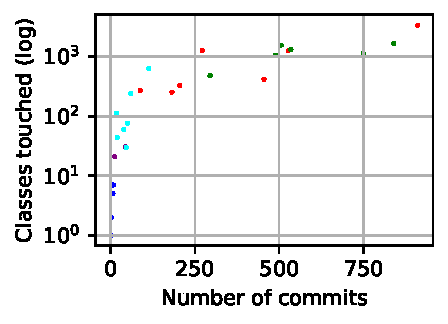
\includegraphics{sections/results/21/classes/sample_scatter_touched_against_commit.classes.sample.first.pdf}
    \caption{classes}
    \label{figure.sections/results/21/classes/sample_scatter_touched_against_commit.classes.sample.first.pdf}
  \end{subfigure}
  \begin{subfigure}[b] 
{0.45\textwidth}
    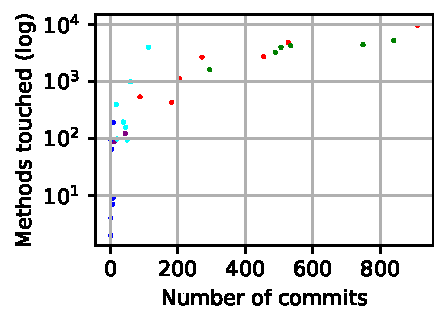
\includegraphics{sections/results/21/methods/sample_scatter_touched_against_commit.methods.sample.first.pdf}
    \caption{methods}
    \label{figure.sections/results/21/methods/sample_scatter_touched_against_commit.methods.sample.first.pdf}
  \end{subfigure}
\caption[Short]{\begin{minipage}[t]{\linewidth}Scatter plots of the log total number of components touched (y-axis) against the number of commits (x-axis) made by samples of developers capped at 84 sustained later joiners from six (6) categories: \color{Blue}Transient Founder (Blue, NUM1), \color{Purple}Moderate Founder (Purple, 3), \color{Green} Sustained Founder (Green, 7), \color{Orange} Transient Later Joiner (Orange, 84), \color{Cyan}Moderate Later Joiner (Cyan, 84), \color{Red} Sustained Later Joiner (Red, 84). \color{Black}\end{minipage}} 
\end{figure}
\clearpage 
